
%%\usepackage[margin=1.5in]{geometry}
%
%% \usepackage{algorithm2e}
%% \usepackage{enumitem}
%% \usepackage{filecontents}
%% \usepackage{todonotes}
%% \usepackage{graphicx}
%\usepackage{subcaption}
%% \usepackage{longtable}
%% \usepackage{booktabs}
%\usepackage{wrapfig}
%% \usepackage[numbers]{natbib}
%%\usepackage{algorithm}
%%\usepackage{algorithmic}
%
%\usepackage{amsmath,amssymb,amsfonts,bm,url,dsfont,hyperref,color}
%%\usepackage[margin=1in]{geometry}
%\newcommand{\kevin}[1]{{\textcolor{red}{#1}}}
%\newcommand\tab[1][1cm]{\hspace*{#1}}
%\newcommand{\polylog}{{\rm polylog}}
%
%\def\calD{\mathcal{D}}
%\def\calE{\mathcal{E}}
%\def\H{\mathcal{H}}
%\def\calS{\mathcal{S}}
%\def\calI{\mathcal{I}}
%\def\S{\mathcal{S}}
%\def\A{\mathcal{A}}
%\def\E{\mathbb{E}}
%\def\1{\mathbf{1}}
%\def\P{\mathbb{P}}
%\def\R{\mathbb{R}}
%\def\mualpha{\mu^{(\alpha)}}
%\newcommand{\mc}[1]{\mathcal{#1}}
%\newcommand{\mbb}[1]{\mathbb{#1}}
%\newcommand{\mbf}[1]{\mathbf{#1}}
%
%%\newtheorem{theorem}{Theorem}
%%\newtheorem{lemma}{Lemma}
%%\newtheorem{remark}{Remark}
%\newtheorem{assumption}{Assumption}
%%\newtheorem{definition}{Definition}

%\setlength{\parindent}{0in}
%\setlength{\parskip}{.5em}

% Heading arguments are {volume}{year}{pages}{date submitted}{date published}{paper id}{author-full-names}

%\jmlrheading{1}{2000}{1-48}{9/18}{10/00}{aziz18a}{Maryam Aziz and Kevin Jamieson and Javed Aslam}
%
%% Short headings should be running head and authors last names
%
%\ShortHeadings{Pure-Exploration for Infinite-Armed Bandits with General Reservoirs}{Aziz, Jamieson, Aslam}
%\firstpageno{1}

%\usepackage[utf8]{inputenc}

%\begin{document}

%\title{Pure-Exploration for Infinite-Armed Bandits with General Arm Reservoirs}

%\author{\name Maryam Aziz \email azizm@ccs.neu.edu \\
%\addr College of Computer and Information Sciences \\
%Northeastern University \\
%Boston, MA 02115, USA
%\AND
%\name Kevin Jamieson \email jamieson@cs.washington.edu \\
%\addr Paul G. Allen School of Computer Science \& Engineering \\
%University of Washington \\
%Seattle, WA 98195, USA
%\AND
%\name Javed Aslam \email jaa@ccs.neu.edu \\
%\addr College of Computer and Information Sciences \\
%Northeastern University \\
%Boston, MA 02115, USA 
%}
%
%\editor{}
%
%
%\maketitle

%\begin{abstract}%   <- trailing '%' for backward compatibility of .sty file
Similar to Chapter~\ref{fixedconfidence}, we consider a multi-armed bandit game where the number of arms is much larger than the maximum, but fixed, budget and is effectively infinite.
In such situations, the sample complexity depends on $\epsilon, \delta$ and the so-called reservoir distribution $\nu$ from which the means of the arms are drawn iid. 
While a substantial literature has developed around analyzing specific cases of $\nu$ such as the beta distribution, our algorithm makes no assumption about the form of $\nu$. It takes a surprising approach that empirically matches or outperforms all state-of-the-art algorithms. 
Our algorithm is based on successive halving with the surprising exception that arms start to be discarded after just a single pull. We present exhaustive experiments in this chapter. We are currently working on proving the correctness of this algorithm.
%\end{abstract}

%\begin{keywords}
%  Infinite-armed bandit, pure-exploration, best-arm identification
%\end{keywords}

% In Section~\ref{experiments} we discuss our  experimental results of using \texttt{Sequential Halving} for pure exploration of the infinitely armed bandits and in Section~\ref{theory} we analyze the simple regret of the algorithm.
%!TEX root = main.tex

\subsection{Introduction}\label{intro}
Consider a multi-armed bandit problem with $n$ arms where the $j$th pull from the $i$th arm emits an independent random variable $X_{i,j} \in [0,1]$ with $\mu_i:=\E[X_{i,j}]$. 
Given $\epsilon,\delta \in (0,1)$, how many total pulls must an algorithm make in order to return an arm $\widehat{i} \in \{1,\dots,n\}$ with a \emph{small}\footnote{While non-standard in stochastic bandits, seeking small means significantly simplifies notation in the infinite-armed bandit setting; we translate all prior results to this equivalent perspective.} mean that satisfies $\mu_{\widehat{i}} \leq \displaystyle\min_{j} \mu_j + \epsilon$ with probability at least $1-\delta$?
Much effort has gone into answering this and closely related questions resulting in a rich collection of algorithms.
But each algorithm starts the same:  \textit{Pull each arm $i \in \{1,\dots,n\}$ once.}
% \begin{quote}

% \centerline{}
% \end{quote}
%
%
\begin{wrapfigure}{r}{0.45\textwidth}
% \vspace{-2.5em}
\includegraphics[width=.45\textwidth]{fixedbudget/figures/folder5/new_yorker.png}
\caption{$3,795$ arms. Difference of the recommended and optimal arm's mean as a function of total pulls. }
\label{fig:newyorker}
\vspace{-1.5em}
\end{wrapfigure}
%
%

In this work we are interested in problems where the number of arms $n$ is so large that it is dwarfed by any available budget of total pulls. Furthermore, we make no assumptions about the so-called arm reservoir.
Necessarily, we are interested in problems where the budget necessary to identify an $\epsilon$-good arm among the $n$ arms with probability $1-\delta$ is \emph{independent} of $n$. 
% Ignoring $\log\log$ factors, it is known that $B = O\left( \sum_{i=1}^n \max\{ (\mu_1 - \mu_i)^{-2}, \epsilon^{-2} \} \right)$ total pulls are \emph{sufficient}.
 % which one notes is always $\Omega(n)$ scaling at least linearly with the number of arms $n$. 
% While \emph{sufficient}, we show that this $\Omega(n)$ number of samples may be far from \emph{necessary}, and that in many natural situations $B$ need not have any dependence on $n$!
% Indeed, this work studies the case when $n \gg B$, that is, when the number of arms $n$ far exceeds the allowable total number of pulls $B$.
Such cases arise when the proportion of $\epsilon$-good arms is independent of $n$ (e.g. $\frac{1}{n} \sum_{i=1}^n \1\{ \mu_i \leq \min_j \mu_j + \epsilon\} \geq \epsilon^2$).

Consider a concrete example of the New Yorker caption contest dataset,
where captions are voted on to find the funniest one (see Section~\ref{experiments}).
The bold blue line is the best-arm identification algorithm lil'UCB \citep{Jamieson2014lilU} executed on all $3,795$ arms, lil'UCB-$X$ for $X$ in $\{10,100,1000,10000\}$ is lil'UCB run on $X$ arms randomly drawn with replacement from the $3,795$ arms, and ISHA is the proposed algorithm of this work. Each algorithm outputs the empirical best arm at any given total budget of pulls, breaking ties randomly.
We observe that one can identify a ``pretty good'' arm faster when the number of drawn arms $X$ is small, but as a consequence this small set of arms will not have an arm very close to the best possible arm.
We also observe that ISHA appears to naturally navigate this tradeoff.  

When $n \gg T$ we can treat $n$ as effectively \emph{infinite} and the difference between sampling an arm with or without replacement is indistinguishable. 
Towards this end, we define the \emph{infinite-armed bandit problem}.

\subsubsection{The Pure-exploration Infinite-armed Bandit Problem}
Let $\nu_0$ be a fixed but arbitrary cumulative distribution function over $\R$ such that if $\boldsymbol{\mu} \overset{iid}{\sim} \nu_0$ then $\P(\boldsymbol{\mu} \leq x) = \nu_0(x)$. 
In the finite-armed bandit case like the example of the previous section, one would take $\nu_0(x) = \frac{1}{n} \sum_{i=1}^n \1\{\mu_i \leq x \}$.
Without loss of generality $\{\mu_i\}_{i=1}^\infty$ are drawn i.i.d. from $\nu_0$ before the start of the game and identified by their index, and the player has no prior knowledge of $\nu_0$.
Consider the pure-exploration infinite-armed bandit game.

\begin{figure}
\centering
\fbox{
	\begin{minipage}{.95\textwidth}
	\textbf{Pure-exploration Infinite-armed bandit game}
	\hrule
	\vspace*{.05in}
	\textbf{Input} $\epsilon,\delta \in (0,1)$ and reservoir distribution $\nu_0$\\
	\textbf{Initialize} Draw $\{\mu_i\}_i \overset{iid}{\sim} \nu_0$ 
	    and set $N_i(t) := \sum_{s=1}^t \1\{I_s = i\}$ for all $t \in \mathbb{N}$\\
	\textbf{for} $t=1,2,\dots$\\
	\hspace*{.25in} Player chooses $I_t \in \mathbb{N}$ \\
	\hspace*{.25in} Nature reveals $X_{I_t,N_{I_t}(t)} \in \R$ 
	    where $\E[X_{I_t,N_{I_t}(t)} | I_t ] = \mu_{I_t}$ \\
	\hspace*{.25in} Player recommends $J_t \in \mathbb{N}$
	\end{minipage}
}
\vspace{-.25in}
\end{figure}
% If $Z_t := X_{I_t,N_{I_t}(t)}$ then given the filtration $\mathcal{F}_t = ( (I_1, Z_1, J_1), \dots, (I_t, Z_t, J_t))$ we have that $I_t$ is $\mc{F}_{t-1}$ measurable, $Z_t$ is $\mc{F}_t$ measureable, and $J_t$ is $\mc{F}_t$ measureable.


\noindent\textbf{Goal:} For a fixed reservoir distribution $\nu_0$ with $\mu_* = \inf \{ x : x \in \text{support}(\nu_0) \}$ and $\epsilon \in (0,1)$, how big must $\tau \in \mathbb{N}$ be to ensure that $\mu_{J_\tau} \leq \mu_* + \epsilon$ with high probability?

\noindent Said another way, minimize \emph{simple regret} \citep{bubeck2009pure,DBLP:journals/corr/CarpentierV15} in high probability, which implies a bound on $\E[\mu_{J_t}]-\mu_*$.

% An important deviation of this simple regret objective from the fixed confidence setting of PAC-learning for multi-armed bandits \cite{EvenDaral06,DBLP:conf/icml/KalyanakrishnanTAS12,icml2013_karnin13,Jamieson2014lilU} is that in the defined infinite armed-bandit problem \emph{the player never decides to stop and output an arm}.
% Suppose the player \emph{did} stop at some finite time under some distribution $\nu$. 
% Because the player has no knowledge of $\nu$, an adversary could look at the player's algorithm and cook up an alternative distribution $\nu'$ that has a very tiny amount of mass near $-\infty$ such that the player would never observe it and be unable to distinguish $\nu$ versus $\nu'$, stop early, and never output an $\epsilon$-good arm. 
% Such an example precisely explains why \emph{finite-armed bandit lower bounds with stopping times} necessarily scale like $\Omega(n)$ \cite{kaufmann2016complexity,simchowitz2017simulator}: the player must sample each arm a minimum number of times to rule it out as $\epsilon$-good.
% Of course, a sample complexity $\Omega(n)$ is meaningless in the infinite-armed bandit when $n$ is infinity, hence, we focus on simple regret \cite{bubeck2009pure,DBLP:journals/corr/CarpentierV15} versus PAC.

% We stress that there are many related and previous works that address different infinite-armed bandit settings that are reviewed in Section~?.
% However, to the best of our knowledge this particular pure-exploration objective in its full generality (e.g., arbitrary reservoir distribution $\nu$) is novel.  



\subsubsection{Prior work}\label{prior_work}

The main objective of this work is \emph{pure-exploration} where different arms are sampled different numbers of times with the goal of choosing $J_t$ after $t=T$ rounds such that the \emph{simple regret} $\mu_{J_t}-\mu_* \leq \epsilon$ for as small $\epsilon$ as possible. 
Contrast this with \emph{exploration-vs-exploitation} where the objective is to pull different arms to minimize the \emph{cumulative regret} of all the plays of the arms pulled: $\sum_{s=1}^t \mu_{I_s} - \mu_*$.
In pure-exploration the player is only evaluated on the mean $\mu_{J_t}$ of the recommended arm at time $t$; in exploration-vs-exploitation the player is evaluated on all the arms played $\{ \mu_{I_s} \}_{s=1}^t$ up to time $t$. 
The infinite-armed case has also been studied in both the explore-vs-exploit and pure-exploration settings, which we briefly review. 

% Within the pure-exploration literature, two studies have been the focus of study: the \emph{fixed budget} and \emph{fixed-confidence} settings. 
% In the fixed budget setting, given a fixed number of arm pulls the objective is to
% either minimize the simple regret (defined above) or the probability of the strategy not returning the best arm.  In the fixed-confidence setting, the objective is
% to find the best arm W.H.P. using as few total arm-pulls as possible.
% The present work is in the fixed budget pure exploration setting where the number of arms is  infinite.
% To provide context, we will next review the literature in the aforementioned settings.

\paragraph{Explore-vs-Exploit: Minimizing cumulative regret.} 

While research on the finite-armed bandit problem for explore-vs-exploit is quite mature \citep{bubeck2012regret}, many open problems still remain for the infinite-armed setting.
To the best of our knowledge, a form of the infinite armed bandit problem was first proposed in \citet{berry1997} which studies the particular case when observations are Bernoulli and $\nu_0$ is the uniform distribution over a known interval $[a,b] \subseteq [0,1]$, but also considers asymptotic upper bounds for their novel algorithm for a more general class of distributions $\nu_0$. 
This work inspired a number of followup works including \cite{teytaud2007anytime} that extended the algorithm of \cite{berry1997} to settings where the time horizon of the algorithm was unknown in advance.  
These algorithms worked on the principle of flipping a coin until $m$ failures are observed at which time it would discard the current coin and sample a new one from $\nu_0$. 
\cite{bonald2013two} studied a related algorithm for Bernoulli observations where $\nu_0$ is a beta distribution:
\begin{align}\label{eqn:beta_distribution}
\nu(\mu) = \int_{\theta=0}^\mu \tfrac{\Gamma(\alpha_1+\alpha_2)}{\Gamma(\alpha_1) \Gamma(\alpha_2)} \theta^{\alpha_1-1}(1-\theta)^{\alpha_2-1} d\theta
\end{align}
with known parameters $\alpha_1,\alpha_2$; lower bounds are proven for any algorithm in this setting.
Note that \eqref{eqn:beta_distribution} with $\alpha_1=\alpha_2=1$ is just the uniform distribution.

While these previous algorithms assumed that $\nu_0$ was equal to some known parameterization of a beta distribution on a known support, \cite{wang2008} relaxed these conditions to simply assume there exists (known) constants $c,C,\beta,\epsilon_0$ such that 
\begin{align} \label{eqn:beta_parameterization}
c \epsilon^\beta \leq \nu_0(\mu_* + \epsilon) \leq C \epsilon^\beta \qquad \forall \epsilon \leq \epsilon_0.
\end{align}
Clearly, for sufficiently small $\epsilon_0$ the beta distribution of \eqref{eqn:beta_distribution} satisfies \eqref{eqn:beta_parameterization} with $\mu_*=0$ and $\beta = \alpha_1$.
In this more general setting \cite{wang2008} proposed an algorithm with cumulative regret guarantees that only needed to know $\beta$, not the support or $\mu_*$.
\citet{Chan2018Infinite} recently proved lower bounds and proposed an algorithm based on confidence intervals.
% And \cite{li2017infinitely} studied another variant under \eqref{eqn:beta_parameterization} where arms have different costs to pull.
To our knowledge, there exists no algorithm in the regret setting that provably adapts to general, unknown reservoir distributions $\nu_0$ with near-optimal cumulative regret. 

A related problem is when each arm's reward distribution is a single-point distribution, or deterministic, but unknown until it is played.
In this setting \cite{david2014infinitely,david2015refined} studied reservoir distributions with conditions similar to \eqref{eqn:beta_parameterization}.

Quantiles are a convenient object in infinite armed bandits since one can very accurately determine how many arms must be sampled to obtain at least one in the $q$th quantile without knowing anything about $\nu_0$. 
% Contrast this with our setting where it is impossible a priori without knowledge of $\nu_0$ to know how many arms must be sampled to obtain one within $\epsilon$ of $\mu_*$. 
In the quantile-regret minimization setting where $\mu_q$ denotes the $q$th percentile of $\nu_0$ for any $q \in (0,1)$, \cite{chaudhuriquantile} provide an algorithm that obtains sub-linear regret with respect to $\mu_q$ (instead of $\mu_*$) for arbitrary reservoir distributions $\nu_0$.

\paragraph{Pure exploration: Simple regret, fixed budget, fixed confidence.}
% Similarly, the finite-armed pure-exploration setting is quite mature and has been studied under a number of metrics which we briefly review. 
% \citet{bubeck2009pure} studied algorithms and limits on the behavior of \emph{simple regret} $\mu_{J_t}-\mu_*$ as a function of $t$. 
% In the \emph{fixed budget} setting \cite{DBLP:conf/colt/AudibertBM10}, the algorithm takes a budget $B$ as input and outputs a single arm $\widehat{i} \in [n]$ and the algorithm is evaluated based on the rate at which $\P( \widehat{i}_B \neq \min_j \mu_j)$ decreases to zero as a function of $B$. 
% The Successive Halving algorithm for the fixed budget setting was proposed in \cite{icml2013_karnin13} which the current work borrows for its algorithm with a particular parameterization.
% One notes that one can trivially obtain simple-regret guarantees from a fixed-budget algorithm.
% Lower bounds were proved for the fixed budget setting in \cite{carpentier2016tight}.
% Finally, in the \emph{fixed confidence (or PAC)} setting the algorithm takes $\delta,\epsilon>0$ as input and attempts to minimize the number of samples before outputting an arm within $\epsilon$ of the best possible with probability at least $1-\delta$ \cite{EvenDaral06, DBLP:conf/icml/KalyanakrishnanTAS12,NIPS2012_4640, icml2013_karnin13,Jamieson2014lilU}. Lower bounds on the sample complexity for this finite bandit problem are also known \cite{Mannor04thesample,kaufmann2016complexity}. 


The infinite-armed bandit setting for pure-exploration is also well-studied. 
The most-biased coin problem is a particular instance where 
\begin{align}\label{eqn:mostbiasedcoin_reservoir}
\nu_0(\mu) = \int_{\theta=0}^\mu \pi \delta_{\rho}(\theta) + (1-\pi) \delta_{\rho+\epsilon}(\theta) \, d\theta
\end{align} 
where $\delta_{x}(\theta)$ is a Dirac-delta at $x$ and parameters $\rho,\pi,\epsilon \in (0,1)$ are known \citep{chandrasekaran2014finding,malloy2012quickest} and unknown \citep{jamieson2016power}.
This parameterization is thought to be difficult because there is no incremental improvement towards the optimal arm over time: the optimal arm has either been identified or it has not. 
 % knowledge of the means of sub-optimal arms provides no knowledge about the value of the optimal mean in the sense that \eqref{eqn:beta_parameterization} does by being able to extrapolate\footnote{This property was used by \cite{DBLP:journals/corr/CarpentierV15} to adapt to unknown $\beta$ in the model of \eqref{eqn:beta_parameterization}.}.
Quantile problems have also been studied in the pure-exploration setting, such as identifying an arm $\epsilon$-close to $\mu_q$ \citep{chaudhuri2017pac,aziz2018pure,ren2018exploring}.



% However, in this setting one finds algorithms that are more robust to uncertainty in the form of reservoir distribution $\nu_0$.
\citet{DBLP:journals/corr/CarpentierV15} proposed an algorithm 
known as SIRI
specifically for  reservoir distributions parameterized as \eqref{eqn:beta_parameterization}.
Remarkably, they show that they can adapt to unknown parameters of this parametric model achieving a simple regret guarantee of  $r_t=\mathcal{O}\left( \max\left(t^{-1/2}, t^{-1/\beta}\polylog(t)\right)\right)$ with high probability for their algorithm; they also provide nearly-matching lower bounds on simpler regret for the $\beta$-parameterization of \eqref{eqn:beta_parameterization}.
\citet{li2017hyperband} proposed the Hyperband algorithm which, to our knowledge, is the only algorithm to obtain simple regret guarantees for general, unknown reservoir distributions (i.e., without a known parameterization like \eqref{eqn:beta_distribution}-\eqref{eqn:mostbiasedcoin_reservoir} of any kind).
For any $\epsilon>0$ and reservoir distribution $\nu_0$, they show that the simple regret of Hyperband is bounded by $\epsilon$ with high probability once the budget $t$ exceeds 
\begin{align}\label{eqn:rough_sample_complexity}
\epsilon^{-2} + \tfrac{1}{\nu_0(\mu_* + \epsilon)}\int_{\mu_*+\epsilon}^\infty \tfrac{1}{(\mu-\mu_*)^2} d\nu_0(\mu)
\end{align}
pulls (up to poly-logarithmic factors).
This result matches all known pure-exploration upper bounds, even those algorithms designed for specific reservoir distributions, up to poly-logarithmic factors.
For any given value of $n \in \mathbb{N}$, Hyperband is nothing more than running $\log_2(n)$ copies of the Successive Halving algorithm of \cite{icml2013_karnin13} each with a budget of $n$ and $2^k$ arms drawn from $\nu_0$ for $k=1,2,\dots,\log_2(n)$; the whole procedure uses $n \log_2(n)$ total samples. 
While Hyperband is state-of-the-art, hedging over these $\log_2(n)$ copies of Successive Halving is inelegant, and empirically it was almost always observed that the most aggressive bracket with the most arms worked best. 


\subsubsection{Main Contributions}
In this work we show that running just one version of Successive Halving, named ISHA, with $n$ arms and a budget of $n\log_2(n)$ pulls--where arms start being discarded after being pulled just once--achieves better simple regret performance than the state-of-the-art Hyperband, but the algorithm is considerably simpler.

We further show that our proposed algorithm is not only superior on most reservoir distributions (including those derived from finite-armed problems) but also against algorithms that were designed specifically for the reservoirs we evaluated them on, like parameterizations \eqref{eqn:beta_distribution}-\eqref{eqn:mostbiasedcoin_reservoir}.

We conjecture that for any reservoir distribution $\nu_0$ and $\epsilon,\delta$, and for sufficiently large $n$ this procedure returns an $\epsilon$-good arm with probability at least $1-\delta$.

Our second contribution is an information theoretic \emph{lower bound} for the infinite-armed bandit problem. 
Specifically, for any reservoir distribution $\nu$ and any fixed $\epsilon,\delta \in (0,1)$ we prove a lower bound on the expected number of samples any algorithm must make in order to identify an $\epsilon$-good arm with probability at least $1-\delta$ that depends on $\nu,\epsilon,\delta$. 
The conjectured upper bound and the lower bound match the expression of \eqref{eqn:rough_sample_complexity} up to possible logarithmic factors.  



%!TEX root = main.tex





\subsection{Successive Halving for infinite-armed bandits}\label{theory}
The Successive Halving algorithm of \cite{icml2013_karnin13} is presented in Figure~2: our proposed algorithm sets $T=\lceil n\log_2(n)\rceil$ for any $n \in \mathbb{N}$.
In what follows of this paper, any reference to Successive Halving should be interepretted as taking the particular parameterization of $T=\lceil n \log_2(n) \rceil$ for any $n \in \mathbb{N}$, unless otherwise specified.
In words, our proposed algorithm is simple: for some $n \in \mathbb{N}$, the algorithm draws $n$ arms without replacement, pulls each arm once, discards the worst half, and on each successive round pulls the surviving arms twice as many times as the previous round before discarding the worst half. The whole process takes $n$ pulls per round for $\log_2(n)$ rounds for a total of $n \log_2(n)$ total pulls.

\begin{figure}[h]
\centering
\fbox{
\begin{minipage}{.95\textwidth}
\textbf{Input}: Budget $T$, number of arms $n$\\
\textbf{Initialization}: Draw $n$ arms and add them to $S_0$\\
% $S_0 \leftarrow \{q_1, \dots, q_n\}$;\\ 
\textbf{For} $k=0,1,\dots, \lceil\log_2(n)\rceil-1$\\
    \hspace*{.15in} Pull each arm $i \in S_k$ for $t_k = \left\lfloor\frac{T}{|S_k|\lceil\log_2(n)\rceil}\right\rfloor$ times and compute empirical means $\widehat{\mu}_{i,k}$ \\
    % let $\hat q_i^r$ be the empirical mean reward of coin $i$; \\
    \hspace*{.15in} Set $S_{k+1}$ to be $\lceil|S_k|/2\rceil$ arms with the lowest empirical means $\widehat{\mu}_{i,k}$ \\
\textbf{Return} Single arm in $S_{\lceil{\log_2(n)}\rceil}$ 
% \end{algorithm}
\end{minipage}
}
\caption{Successive Halving algorithm. The algorithm we propose for infinite-armed bandits is to use $T = \lceil n \log_2(n) \rceil$ for any value of $n \in \mathbb{N}$. For anytime, double $n$ and repeat.}\label{alg-SH}
\end{figure}

The main dilemma of choosing $X$ for the lil'UCB-$X$ strategies in the introduction of this paper, and more generally all infinite-armed bandit problems, is determining whether it is better to draw more arms from a reservoir distribution over arms in the hope of getting an arm with better mean reward, or to spend the remaining arm pull budget on identifying a ``good'' arm from among already drawn arms.
Our proposed parameterization of Sequential Halving navigates this dilemma by focusing not on individual arms but on populations of arms, where at each round the ``fitter'' (i.e. lower empirical mean) arms are more likely to survive and so from round to round the population as a whole ``evolves,'' in the sense that while any individual ``good'' arm might get unlucky and be removed from the population, overall the average expected reward of the surviving arms tends to improve.
% By allocating budget uniformly in each round of the algorithm to the
% arms with highest empirical means from the last round,
% it naturally avoids spending too much budget on arms which, on the one
% hand, are already performing better than the majority of the population
% and do not yet need further testing,
% or, on the other hand, have performed much worse than the majority of arms and can safely be eliminated.



% Suppose $n$ arms are drawn such that $\mu_i \sim \nu_0$ for $i=1,\dots,n$ and placed in a set $S_0$. 
% At round $k$, each arm $i \in S_k$ is sampled $2^k$ times to obtain an empirical mean $\widehat{\mu}_{i,k}$. 
% The set $S_{k+1}$ is defined to contain the $|S_k|/2 = n 2^{-k}$ arms with the smallest empirical means (breaking ties arbitrarily). 

% Note that at each round $k$ we have $|S_k| = n 2^{-k}$.
% And if 
% \begin{align*}
% n = \arg\max\{ n' \in \mathbb{N} : n' \lceil \log_2 (n') \rceil \leq T \}
% \end{align*}
% then each $t_k = 2^k$. 
% This choice of $n$, given a budget $T$, is the algorithm we will analyze.
% It is remarkable that on the first round, $k=0$, each coin is sampled just a \emph{single} time before half the arms are discarded. 





% Also define
% \begin{align*}
% F_k(x,\mu) = \P\left( \widehat{\mu}_{i,k} \leq x \, | \, \E[\widehat{\mu}_{i,k}] = \mu \right) \quad \text{ and } \quad F_k(x) = \E\left[ \tfrac{1}{|S_k|}\sum_{i \in S_k} \1\{ \widehat{\mu}_{i,j} \leq x) \} \right] = \int F_k(x,\mu) d\nu_k(\mu).
% \end{align*}
% Note that $F_0(x,\mu)$ is the CDF of a single draw of a random variable with mean $\mu$. 
% Likewise, $F_k(x,\mu)$ is equal to $F_0(x,\mu)$ convolved with itself $2^k$ times.
\subsubsection{Analysis}
Our main result relies on two assumptions about the distribution $\phi(\ \cdot \ ; \mu)$ of observations from an arm given a drawn mean $\mu$.
We make no assumptions about the shape or regularity of the reservoir $\nu_0$.
% For instance, $\phi(\mu) = \mathcal{N}(\mu,1)$ or $\phi(\mu) = \text{Bernoulli}(\mu)$. 
\begin{assumption} \label{asm:stochastic_ordering}
% Let $\phi(\mu)$ denote the probability law that observations from an arm with mean $\mu$ obey. 
For all $m \in \mathbb{N}$ and $t \in \R$
\begin{align*}
\P\Big(\frac{1}{m} \sum_{j=1}^m X_j \leq t \, \Big| \, X_j \overset{iid}{\sim} \phi( \ \cdot \ ; x) \Big) \geq \P\Big(\frac{1}{m} \sum_{j=1}^m Y_j \leq t \, \Big| \, Y_j \overset{iid}{\sim} \phi( \ \cdot \ ; y) \Big) \iff x \leq y.
\end{align*} 
\end{assumption}
Assumption~\ref{asm:stochastic_ordering} states that the distribution with the smaller mean is more likely to have a smaller empirical mean. 
This holds, for example, if $\phi(\cdot,\mu)$ is $\text{Bernoulli}(\mu)$ or Gaussian observations with known variance $\mathcal{N}(\mu,R)$.
A consequence of Assumption~\ref{asm:stochastic_ordering} is that
\begin{align*}
\P( \mu_i \in S_{k+1} \, | \, \mu_i = x, \mu_i \in S_{k} ) \geq \P( \mu_i \in S_{k+1} \, | \, \mu_i = y, \mu_i \in S_{k} ) \quad \forall x \leq y.
\end{align*} 
Assumption~\ref{asm:stochastic_ordering} often holds for the class of single-parameter exponential families that are well-studied in the multi-armed bandit literature \citep{audibert2010best}.
Our second assumption is standard and allows us to rely on the concentration of measure phenomenon.
\begin{assumption}\label{asm:subgauss}
If $X \sim \phi(\ \cdot \ ; \mu)$ then $X-\mu$ is an i.i.d. mean-zero, $R$-sub-Gaussian random variable such that $\E[\exp(\lambda (X-\mu))] \leq \exp(\lambda^2 R /2 )$ for any $\lambda >0$.
\end{assumption} 
Assumption~\ref{asm:subgauss} is quite benign: if $X \in [0,1]$ then $R \leq 1/4$; if $X \sim \mathcal{N}(\mu,v^2)$ then $R = v^2$.

\begin{theorem}\label{thm:main}
Fix $\delta \in (0,1)$. Under Assumptions 1 and 2, for any $\epsilon >0$ define
\begin{align*}
z_{n,\epsilon} :=& \frac{\log(2 \log_2(n)/\delta)}{  \nu_0(\mu_* + \epsilon)} \max\left\{ 1, 64 R \log(4 n \log_2(n) /\delta) \sup_{x \geq \mu_* + \epsilon}  (x-\mu_*)^{-2}  \nu_0(x) \right\}\\
\leq& \log(2 \log_2(n)/\delta) \max\Bigg\{ \frac{1}{\nu_0(\mu_* + \epsilon)},
\\ &~~~~~~~~~~
64 R \log(4 n \log_2(n) /\delta) \left( \epsilon^{-2} + \frac{1}{\nu_0(\mu_* + \epsilon)}\int_{x = \mu_* + \epsilon}^\infty  \frac{1}{(x-\mu_*)^{2}}  d\nu_0(x) \right) \Bigg\}.
\end{align*}
If Successive Halving of Figure~\ref{alg-SH} is run with $n$ arms and $T=\lceil n \log_2(n) \rceil$ total pulls where $n \geq z_{n,\epsilon}$ then with probability at least $1-\delta$ the single arm returned is no greater than $\mu_* +\epsilon$.
\end{theorem}
% \begin{theorem}\label{thm:main}
% Fix $\delta \in (0,1)$ and assume Assumptions 1 and 2 hold.
% Define 
% \begin{align*}
% \Delta_\ell := 2\sqrt{\frac{2R \log(n \log_2(n) 2^{-\ell+2}/\delta)}{2^\ell}} \ , \qquad\qquad \forall \ell \in \{0,1,\dots,\log_2(n)-1\}.
% \end{align*}
% If 
% \begin{align*}
% n \geq z_n :=& \max_{k=0,1,\dots,\log_2(n)-1} \frac{\log(2 \log_2(n)/\delta)}{  \nu_0(\mu_* + \Delta_k)} \max\{ 1, \max_{\ell=0,\dots,k-1} 2^{\ell+1} \nu_0(\mu_* + 2\Delta_{\ell}) \}
% \end{align*}
% then with probability at least $1-\delta$
% \begin{align*}
% \mu_{A} \leq  \min_{i \in S_k} \mu_i + \Delta_k/2 \leq \mu_* + \tfrac{3}{2} \Delta_k \quad \text{where} \quad A = \arg\min_{i \in S_k} \widehat{\mu}_{i,k}
% \end{align*} 
% for all $k = 0, 1, \dots, \log_2(n)-1$.
% \end{theorem}
% We can make the theorem more interpretable by simplifying $z_n$
% \begin{align*}
% \max_{\ell=0,\dots,k-1}  2^{\ell+1} \nu_0(\mu_* + 2\Delta_{\ell}) &= \max_{\ell=0,\dots,k-1}  16 R \log(n \log_2(n) 2^{-\ell+2}/\delta) \Delta_{\ell}^{-2}  \nu_0(\mu_* + 2\Delta_{\ell}) \\
% &\leq  64 R \log(4 n \log_2(n) /\delta) \max_{\ell=0,\dots,k-1}  (2\Delta_{\ell})^{-2}  \nu_0(\mu_* + 2\Delta_{\ell}) \\
% &\leq  64 R \log(4 n \log_2(n) /\delta) \sup_{x \geq \mu_* + \Delta_{k-1}}  (x-\mu_*)^{-2}  \nu_0(x).
% \end{align*}
% We note that
% \begin{align*}
% \max_{k=0,1,\dots,\log_2(n)-1} &\frac{\log(2 \log_2(n)/\delta)}{  \nu_0(\mu_* + \Delta_k)} \max\{ 1, \max_{\ell=0,\dots,k-1} 2^{\ell+1} \nu_0(\mu_* + 2\Delta_{\ell}) \}\\
% \leq& \max_{k=0,1,\dots,\log_2(n)-1} \frac{\log(2 \log_2(n)/\delta)}{  \nu_0(\mu_* + \Delta_k)} \max\left\{ 1, 64 R \log(4 n \log_2(n) /\delta) \sup_{x \geq \mu_* + \Delta_{k-1}}  (x-\mu_*)^{-2}  \nu_0(x) \right\} \\
% \leq& \frac{\log(2 \log_2(n)/\delta)}{  \nu_0(\mu_* + \Delta_{\log_2(n)-1})} \max\left\{ 1, 64 R \log(4 n \log_2(n) /\delta) \sup_{x \geq \mu_* + \Delta_{\log_2(n)-1}}  (x-\mu_*)^{-2}  \nu_0(x) \right\}
% \end{align*}

% If we set $\epsilon = \Delta_{\log_2(n)-1}$ and define 
% \begin{align*}
% z_{n,\epsilon} :=& \frac{\log(2 \log_2(n)/\delta)}{  \nu_0(\mu_* + \epsilon)} \max\left\{ 1, 64 R \log(4 n \log_2(n) /\delta) \sup_{x \geq \mu_* + \epsilon}  (x-\mu_*)^{-2}  \nu_0(x) \right\}\\
% \leq& \frac{\log(2 \log_2(n)/\delta)}{  \nu_0(\mu_* + \epsilon)} \max\left\{ 1,  64 R \log(4 n \log_2(n) /\delta) \left( \epsilon^{-2} \nu_0(\mu_*+\epsilon) + \int_{x = \mu_* + \epsilon}^\infty  \frac{1}{(x-\mu_*)^{2}}  d\nu_0(x) \right) \right\} \\
% =& \log(2 \log_2(n)/\delta) \max\left\{ \frac{1}{\nu_0(\mu_* + \epsilon)}, 64 R \log(4 n \log_2(n) /\delta) \left( \epsilon^{-2} + \frac{1}{\nu_0(\mu_* + \epsilon)}\int_{x = \mu_* + \epsilon}^\infty  \frac{1}{(x-\mu_*)^{2}}  d\nu_0(x) \right) \right\}
% \end{align*}
% then the algorithm outputs an $\tfrac{3}{2}\epsilon$-good arm with with probability at least $1-\delta$ whenever $n \geq z_{n,\epsilon}$.


Before we prove the theorem, we need some notation and technical lemmas.
Define 
\begin{align*}
\nu_k(x) = \E\Big[ \tfrac{1}{|S_k|} \sum_{i \in S_k} \1\{ \mu_i \leq x \} \Big] = \P( \mu_i \leq x \, | \, \mu_i \in S_k )
\end{align*}
where the expectation is taken with respect to the random set $S_k$. 
Note that this definition is consistent with the reservoir distribution $\nu_0( \, \cdot \, )$ for $k=0$.
Also define
\begin{align*}
\Delta_\ell := 2\sqrt{\frac{2R \log(n \log_2(n) 2^{-\ell+2}/\delta)}{2^\ell}} \ , \qquad\qquad \forall \ell \in \{0,1,\dots,\log_2(n)-1\}.
\end{align*}

The next lemma follows by a straightforward union and Chernoff bound (Appendix~\ref{sec:concentration_in_k_proof}).
\begin{lemma}\label{lem:concentration_in_k}
Under Assumption~\ref{asm:subgauss} we have
% \begin{align*}
$\P\left( \bigcup_{\ell=0}^{\log_2(n)-1} \bigcup_{i \in S_{\ell}} \left\{ |\widehat{\mu}_{i,\ell} - \mu_\ell| \geq \Delta_\ell/2 \right\} \right) \leq \delta/2$.
% \end{align*}
\end{lemma}

The next lemma exploits the fact that each $\mu_i \in S_k$ for any $k$ is an iid draw from $\nu_k$, by definition, and $|S_k| = n 2^{-k}$.
The result follows by a union bound over $k$ (Appendix~\ref{sec:good_arms_in_set_k_proof}).
\begin{lemma}\label{lem:good_arms_in_set_k}
For any $\ell=0,1,\dots,\log_2(n)-1$ if  $n \geq \xi_{n,\ell} := \frac{\log(2 \log_2(n)/\delta)}{2^{-\ell} \nu_\ell(\mu_* + \Delta_\ell)}$ then 
% If $n \geq \max_{\ell =0,1,\dots, \log_2(n)-1} \frac{\log(2 \log_2(n)/\delta)}{2^{-\ell} \nu_\ell(\mu_* + \Delta_\ell)}$ then
\begin{align*}
\P\Big(\min_{i \in S_\ell} \mu_i > \mu_* + \Delta_\ell \Big) \leq \tfrac{\delta}{2 \log_2(n)}.
\end{align*}
Moreover, $\P\Big( \bigcup_{\ell=0}^{\log_2(n)-1} \left\{ \min_{i \in S_\ell} \mu_i > \mu_* + \Delta_\ell \right\} \Big)\leq \frac{\delta}{2}$
whenever $n \geq \max_{\ell=0,1,\dots,\log_2(n)-1} \xi_{n,\ell}$.
\end{lemma}


If $n \geq  \max_{\ell=0,1,\dots,\log_2(n)-1} \frac{\log(2 \log_2(n)/\delta)}{2^{-\ell} \nu_\ell(\mu_* + \Delta_\ell)}$, then combining the two above lemmas would give the desired result of Theorem~\ref{thm:main}.
However, $\nu_k$ is not a natural quantity to reason about since it depends on the behavior of the algorithm.
The next two lemmas characterize the behavior of this evolving distribution.
The proof of the following lemma applies Bayes rule and exploits Assumption~\ref{asm:stochastic_ordering}. 
It comes to the intuitive conclusion that the distribution of the true means gets no worse by thresholding the empirical means at the median (Appendix~\ref{sec:core_lemma_proof}).
\begin{lemma}\label{lem:core_lemma}
Assume Assumption~\ref{asm:stochastic_ordering} holds.
For any $k$ and $x\in \R$ we have
\begin{align*}
\nu_{k+1}(x) &= 2 \P( \mu_i \in S_{k+1} \, | \, \mu_i \leq x, \mu_i \in S_{k} ) \, \nu_k(x)
\geq \nu_k(x).
\end{align*}
Moreover, for any $k$ and $x < y$ we have $\frac{\nu_{k+1}(x)}{\nu_k(x)} \geq \frac{\nu_{k+1}(y)}{\nu_k(y)}$.
% \begin{align*}
% \frac{\nu_{k+1}(x)}{\nu_k(x)} \geq \frac{\nu_{k+1}(y)}{\nu_k(y)}.
% \end{align*}
\end{lemma} 

\noindent The next lemma refines the previous one, stating sufficient conditions for  improvement. 
\begin{lemma}\label{lem:E_k}
Assume Assumption~\ref{asm:stochastic_ordering} holds.
Fix some $k \in \mathbb{N}$. 
% Without loss of generality, at stage $k$ we have $\mu_i \sim \nu_k$ for $i \in S_k = \{1,\dots,|S_k|\}$. 
% The realized random variables $\widehat{\mu}_{i,k}$ are the result of averaging $2^k$ realizations from the base distribution with mean $\mu_i$.  
Define the event
\begin{align*}
\mathcal{E}_k = \{ \min_{i\in S_k} \mu_i-\mu_* \leq \Delta_k, \, \max_{i\in S_k} |\widehat{\mu}_{i,k} - \mu_i| \leq \Delta_k/2\}.
\end{align*} 
Then
\begin{align} 
\nu_{k+1}(\mu_*+\epsilon) &\geq \1_{\mathcal{E}_k}\min\{ 1, 2 \nu_k(\mu_*+\epsilon) , \tfrac{\nu_0(\mu_*+\epsilon) }{\nu_0(\mu_* + 2\Delta_k)} \} \quad \forall \epsilon \leq \Delta_k. \label{eqn:recursion}
\end{align}
\end{lemma}
\begin{proof}
Assume $\mathcal{E}_k$.
We consider two exhaustive cases: 

\noindent\textbf{Case 1}: $\max_{i \in S_{k+1}} \widehat{\mu}_{i,k} \leq \mu_* + \Delta_k + (\Delta_k/2)$. Here 
\begin{align*}
\max_{i \in S_{k+1}} \mu_i \leq \max_{i \in S_{k+1}} \widehat{\mu}_{i,k} + \Delta_k/2 \leq \mu_* + 2 \Delta_k
\end{align*} 
which means that no $2\Delta_k$-bad arms make it into $S_{k+1}$ and $\nu_{k+1}(\mu_*+2\Delta_k)=1$. Thus, applying the second result of Lemma~\ref{lem:core_lemma} twice with $x = \mu_* + \epsilon$ and $y=\mu_* + 2 \Delta_k$, we have $\nu_{k+1}(\mu_* + \epsilon) \geq \frac{\nu_k(\mu_*+\epsilon)}{\nu_k(\mu_* + 2\Delta_k)} \geq \frac{\nu_0(\mu_*+\epsilon)}{\nu_0(\mu_* + 2\Delta_k)}$ for all $\epsilon < \Delta_k$.

\noindent\textbf{Case 2}: $\mu_* + \Delta_k + (\Delta_k/2) < \max_{i \in S_{k+1}} \widehat{\mu}_{i,k}$ In this case all $\Delta_k$-good arms in $S_k$ are guaranteed to be in $S_{k+1}$. Thus $\nu_{k+1}(\mu_*+\Delta_k) = \min\{1,2 \nu_{k}(\mu_* + \Delta_k)\}$ by the first result of Lemma~\ref{lem:core_lemma} with $x = \mu_* +\Delta_k$.
% \begin{align*}
% \mathcal{E}_k \implies \nu_{k+1}(\mu_*+\epsilon) &\geq \min\{ 1, 2 \nu_k(\mu_*+\epsilon) , \tfrac{\nu_k(\mu_*+\epsilon) }{\nu_k(\mu_* + 2\Delta_k)} \} \quad \forall \epsilon \leq \Delta_k.
% \end{align*}
\end{proof}

We are now ready to prove Theorem~\ref{thm:main}.
\begin{proof}
Let $z_{n,\Delta_{k}}$ be $z_{n,\epsilon}$ from the theorem statement with $\epsilon=\Delta_k$. Define
% \begin{align*}
% z_{n,\Delta_{k}}&:= \frac{\log(2 \log_2(n)/\delta)}{  \nu_0(\mu_* + \Delta_{k})} \max\left\{ 1, 64 R \log(4 n \log_2(n) /\delta) \sup_{x \geq \mu_* + \Delta_{k}}  (x-\mu_*)^{-2}  \nu_0(x) \right\}
% \end{align*}
% as well as
\begin{align*}
z_n := \max_{k=0,1,\dots,\log_2(n)-1} z_{n,\Delta_{k}}= z_{n,\Delta_{\log_2(n)-1}}  \quad \text{and} \quad
\xi_{n,k} := \frac{\log(2 \log_2(n)/\delta)}{2^{-k} \nu_k(\mu_* + \Delta_k)}
\end{align*}
where $\xi_{n,k}$ comes from Lemma~\ref{lem:good_arms_in_set_k}.
Note that $n \geq z_n$ by assumption.
The theorem claims that with probability at least $1-\delta$ the returned arm has a mean no greater than $\mu_* + \Delta_{\log_2(n)-1}$ (which is implied if $\mathcal{E}_{\log_2(n)-1}$ holds) whenever $n \geq z_n = z_{n,\Delta_{\log_2(n)-1}}$ by simply making the substitution $\epsilon := \Delta_{\log_2(n)-1}$.
Thus, our goal is to show that $\mathcal{E}_{\log_2(n)-1}$ holds by proving the stronger statement that $\bigcap_{k=0}^{\log_2(n)-1} \mathcal{E}_k$ holds.

By immediate application of Lemma~\ref{lem:concentration_in_k} and Lemma~\ref{lem:good_arms_in_set_k}, for all $k=0,1,\dots,\log_2(n)-1$ simultaneously
\begin{align}\label{eqn:main_implication}
\{n \geq \xi_{n,k}\}  \implies \{ \min_{i \in S_k} \mu_i \leq \mu_* + \Delta_k \} \cap  \{ \max_{i\in S_k} |\widehat{\mu}_{i,k} - \mu_i| \leq \Delta_k/2 \} = \mc{E}_k
\end{align}
with probability at least $1-\delta$.
% Thus, since $n \geq z_n$ it suffices to show that $\bigcap_{k=0}^{\log_2(n)-1} \{z_{n,\Delta_k} \geq \xi_{n,k}\}$.
In what follows, assume the implication of \eqref{eqn:main_implication} holds for all $k$, since these occur with probability at least $1-\delta$.

We will prove the theorem by induction
% \begin{align*}
% \{ n \geq z_n \} \cap \left\{ \bigcap_{\ell=0}^{k-1} \mathcal{E}_\ell \right\} \implies \{ n \geq z_n \} \cap \left\{ \bigcap_{\ell=0}^{k} \mathcal{E}_\ell \right\}
% \end{align*}
starting with the base case
\begin{align*}
\{n \geq z_n\} \implies \{ n \geq z_{n,\Delta_0} \} \implies \{ n \geq \frac{\log(2 \log_2(n)/\delta)}{ \nu_0(\mu_* + \Delta_0)} \} \equiv \{n \geq \xi_{n,0}\} \overset{\eqref{eqn:main_implication}}{\implies} \mc{E}_0.
\end{align*} 
Fix any $k \in \{1,\dots,\log_2(n)-1\}$. 
Note $\{\nu_k(\mu_*+\Delta_k)=1 \} \implies \left\{ \min_{i \in S_k} \mu_i-\mu_* \leq \Delta_k \right\}$ so
\begin{align*}
\{\nu_k(\mu_*+\Delta_k)=1 \} \cap \{ \max_{i\in S_k} |\widehat{\mu}_{i,k} - \mu_i| \leq \Delta_k/2 \} \implies \mathcal{E}_k.
\end{align*} 
So assume $\nu_k(\mu_*+\Delta_k)<1$.
On $\left\{ \bigcap_{\ell=0}^{k-1} \mathcal{E}_\ell \right\}$ we have 
\begin{align*}
\nu_{k}(\mu_*+\Delta_k) &\geq \min\{ 1, 2 \nu_{k-1}(\mu_*+\Delta_k) , \tfrac{\nu_0(\mu_*+\Delta_k) }{\nu_0(\mu_* + 2\Delta_{k-1})} \} \\
&\geq \min\{ 1, 2 \min\{ 1, 2 \nu_{k-2}(\mu_*+\Delta_k) , \tfrac{\nu_0(\mu_*+\Delta_k) }{\nu_0(\mu_* + 2\Delta_{k-2})} \} , \tfrac{\nu_0(\mu_*+\Delta_k) }{\nu_0(\mu_* + 2\Delta_{k-1})} \} \\
% &= \min\{ 1, 2^2 \nu_{k-2}(\mu_*+\Delta_k) , 2 \tfrac{\nu_0(\mu_*+\Delta_k) }{\nu_0(\mu_* + 2\Delta_{k-2})} , \tfrac{\nu_0(\mu_*+\Delta_k) }{\nu_0(\mu_* + 2\Delta_{k-1})} \} \\
&\geq \min\{ 1,2^{k} \nu_0(\mu_* + \Delta_k), \min_{\ell=0,\dots,k-1} 2^{k-1-\ell} \tfrac{\nu_0(\mu_*+\Delta_k)}{\nu_0(\mu_* + 2\Delta_{\ell})} \} \\
&= \min\{ 1,2^{k} \nu_0(\mu_* + \Delta_k) \min\{ 1,   \tfrac{1}{\max_{\ell=0,\dots,k-1} 2^{\ell+1} \nu_0(\mu_* + 2\Delta_{\ell})} \} \}\\
% &= 2^{k} \nu_0(\mu_* + \Delta_k) \min\{ 1,   \tfrac{1}{\max_{\ell=0,\dots,k-1} 2^{\ell+1} \nu_0(\mu_* + 2\Delta_{\ell})} \} \\
&= 2^{k} \nu_0(\mu_* + \Delta_k) \tfrac{1}{\max\{ 1, \max_{\ell=0,\dots,k-1} 2^{\ell+1} \nu_0(\mu_* + 2\Delta_{\ell}) \}} 
\end{align*}
where the last line uses $\nu_k(\mu_*+\Delta_k)<1$ and moves the $\min$ to the denominator.
Now
% \begin{align*}
% \max\{1, \max_{\ell=0,\dots,k-1}  2^{\ell+1} \nu_0(\mu_* + 2\Delta_{\ell}) \} &= \max\{1, \max_{\ell=0,\dots,k-1}  16 R \log(n \log_2(n) 2^{-\ell+2}/\delta) \Delta_{\ell}^{-2}  \nu_0(\mu_* + 2\Delta_{\ell}) \} \\
% &\leq \max\{1, 64 R \log(4 n \log_2(n) /\delta) \max_{\ell=0,\dots,k-1}  (2\Delta_{\ell})^{-2}  \nu_0(\mu_* + 2\Delta_{\ell}) \} \\
% &\leq \max\{1, 64 R \log(4 n \log_2(n) /\delta) \sup_{x \geq \mu_* + \Delta_{k-1}}  (x-\mu_*)^{-2}  \nu_0(x) \} \\
% &\leq \max\{1, 64 R \log(4 n \log_2(n) /\delta) \sup_{x \geq \mu_* + \Delta_{k}}  (x-\mu_*)^{-2}  \nu_0(x) \} \\
% &= \frac{\nu_0(\mu_* + \Delta_{k})}{\log(2 \log_2(n)/\delta)} z_{n,\Delta_{k}}.
% % &\leq \frac{\nu_0(\mu_* + \Delta_{k})}{\log(2 \log_2(n)/\delta)} n .
% \end{align*}
\begin{align*}
\max_{\ell=0,\dots,k-1}  2^{\ell+1} \nu_0(\mu_* + 2\Delta_{\ell}) &= \max_{\ell=0,\dots,k-1}  16 R \log(n \log_2(n) 2^{-\ell+2}/\delta) \Delta_{\ell}^{-2}  \nu_0(\mu_* + 2\Delta_{\ell}) \\
&\leq 64 R \log(4 n \log_2(n) /\delta) \max_{\ell=0,\dots,k-1}  (2\Delta_{\ell})^{-2}  \nu_0(\mu_* + 2\Delta_{\ell}) \\
&\leq 64 R \log(4 n \log_2(n) /\delta) \sup_{x \geq \mu_* + \Delta_{k-1}}  (x-\mu_*)^{-2}  \nu_0(x) \\
&\leq 64 R \log(4 n \log_2(n) /\delta) \sup_{x \geq \mu_* + \Delta_{k}}  (x-\mu_*)^{-2}  \nu_0(x),
\end{align*}
% so that
\begin{align*}
\max\{1, \max_{\ell=0,\dots,k-1}  2^{\ell+1} \nu_0(\mu_* + 2\Delta_{\ell}) \}
&\leq \max\{1, 64 R \log(4 n \log_2(n) /\delta) \sup_{x \geq \mu_* + \Delta_{k}}  (x-\mu_*)^{-2}  \nu_0(x)\} \\
&=\tfrac{\nu_0(\mu_* + \Delta_{k})}{\log(2 \log_2(n)/\delta)} z_{n,\Delta_{k}}.
% &\leq \frac{\nu_0(\mu_* + \Delta_{k})}{\log(2 \log_2(n)/\delta)} n .
\end{align*}
Plugging this result back into the previous display and rearranging, we obtain
\begin{align*}
\nu_{k}(\mu_*+\Delta_k) \geq \frac{2^k \log(2 \log_2(n)/\delta)}{z_{n,\Delta_{k}}} \equiv z_{n,\Delta_k} \geq \xi_{n,k}.
\end{align*}
Thus,
\begin{align*}
\{n \geq z_n \} \cap \left\{ \bigcap_{\ell=0}^{k-1} \mathcal{E}_\ell \right\} &\implies \{n \geq z_n \} \cap \{z_{n,\Delta_k} \geq \xi_{n,k} \} \cap \left\{ \bigcap_{\ell=0}^{k-1} \mathcal{E}_\ell \right\}  \overset{\eqref{eqn:main_implication}}{\implies} \{n \geq z_n \} \cap  \left\{ \bigcap_{\ell=0}^{k} \mathcal{E}_\ell \right\}
\end{align*}
Because $k$ was chosen arbitrarily, and because $\mc{E}_0$ holds, we have proven that 
$\{n \geq z_n \} \implies \left\{ \bigcap_{\ell=0}^{\log_2(n)-1} \mathcal{E}_\ell \right\}$ 
with probability at least $1-\delta$.
\end{proof}


\subsection{Lower bound}

Fix any reservoir distribution $\nu_0$ and $\epsilon,\delta \in (0,1)$. 
Our upper bound of Theorem~\ref{thm:main} states that if the proposed algorithm is provided a budget of $\epsilon^{-2}+\frac{1}{\nu_0(\mu_* + \epsilon)}\int_{\mu_*+\epsilon} (\mu-\mu_*)^{-2} d\nu_0(\mu)$ pulls (up to poly-logarthmic factors), then the prescribed procedure outputs an $\epsilon$-good coin with probability at least $1-\delta$.
In this section, we argue that any algorithm that identifies an $\epsilon$-good coin with probability at least $1-\delta$ must take nearly this many total pulls in expectation.
We follow the lower bound technique of \cite{malloy2012quickest} beginning with a definition borrowed from \cite{berry1997}.
\begin{definition}
% Fix any $\nu_0$ and $\epsilon,\delta\in(0,1)$.
A \emph{non-recalling strategy} is one that always draws a new arm from $\nu_0$ when switching from the current arm and never pulls a previous arm again.
% At each time the procedure recommends the arm being currently pulled.  
\end{definition}

Implicit in \cite{malloy2012quickest} is the assumption that there exists a non-recalling strategy for every $\nu_0, \epsilon, \delta$ that is near-optimal with respect to \emph{any} strategy.
Such an assumption is reasonable because observations from any particular arm are conditionally independent given the mean of the arm, and knowing the mean of one arm provides no information about the mean of another. 
Thus, the number of times any particular arm is pulled depends \emph{only} on the observations from that arm, and because the means of the arms are drawn iid from $\nu$, each arm should be treated identically.
Thus, the procedure will continue to discard arms until it finds one and commits to it for all time. 
Of course, any such strategy would require precise knoweldge of $\nu_0$ making it impractical, but it useful for a lower bound.


% The only reason for exploration in bandits is to discover what \emph{else} is out there, but in this case the player knows $\nu$ exactly, so they already \emph{know} what else is out there. 
% Thus, we only need to consider algorithms that act on one arm at a time, and treat each arm identically. 
Define
$KL(\mu,\mu') = \int_{x} \phi(x;\mu) \log\left( \frac{\phi(x;\mu)}{\phi(x;\mu')}\right) dx$
where we assume $KL(c,d) \geq KL(a,b)$ for all $[a,b] \subseteq [c,d]$.
This is a common assumption and holds for families of distributions $\phi( \cdot ; \mu)$ parameterized by their mean (e.g., Bernoulli, Gaussian, Poisson) \cite{kaufmann2016complexity}.
\begin{theorem}
Fix a reservoir distribution $\nu$, $\delta \in (0,1/15)$, and $\epsilon >0$ such that $\nu(\mu_*+\epsilon) \leq 1/2$.
If at time $\tau \in \mathbb{N}$ a non-recalling strategy outputs an arm $\widehat{i} \in \mathbb{N}$ that satisfies $\P(\mu_{\widehat{i}} \leq \mu_* + \epsilon ) \geq 1-\delta$, then
\begin{align*}
\E[ \tau ] &\geq (1-\delta)\frac{  \log(\tfrac{(1-\delta)\widetilde{\kappa}}{e \delta \nu(\mu_*+\epsilon)})}{KL(\mu_* , \widetilde{\mu})}  - \frac{2}{KL(\mu_* + \epsilon, \mu_*)}  + \frac{3/8}{\nu(\mu_*+\epsilon)} \int_{\mu_*+\epsilon} \frac{1}{KL(\mu,\mu_*)} d\nu(\mu) 
\end{align*}
for any $\widetilde{\mu}$ with $\widetilde{\kappa} := \nu(\widetilde{\mu}) - \nu(\mu_*+\epsilon) > \frac{ \delta \nu(\mu_*+\epsilon)}{1-\delta}$
\end{theorem}


\noindent We related this lower bound to previously known upperbounds using Gaussian realizations (or Bernoulli's near $1/2$) where $KL(\mu,\mu') \leq c (\mu-\mu')^2$: 

\noindent\textbf{Continuous as $\mu \rightarrow \mu_*$:} Take $\widetilde{\kappa} = \sqrt{\delta}$. As $\delta \rightarrow 0$ we have $\widetilde{\mu} \rightarrow \mu_*+\epsilon$ to yield a sample compelxity of $\epsilon^{-2} \log(\tfrac{1}{ \delta \nu(\mu_*+\epsilon)}) + \frac{1}{\nu(\mu_*+\epsilon)} \int_{\mu_*+\epsilon} \frac{1}{(\mu-\mu_*)^2} d\nu(\mu)$.

\noindent\textbf{Two spike, Equation~\ref{eqn:mostbiasedcoin_reservoir}:} Take $\widetilde{\kappa} = (1-\pi)$ to yield a sample complexity of $\epsilon^{-2} \log(\tfrac{1}{\pi \delta}) + \frac{1}{\pi \epsilon^2}$.

\noindent\textbf{Polynomial-tail, Equation~\ref{eqn:beta_parameterization}:} $\nu(\mu_* + x) := \P( \mu \leq \mu_* + x) \propto x^\beta$. Take $\widetilde{\mu} = \mu_* + 2^{1/\beta} \epsilon$ so that $\widetilde{\kappa} = \nu(\mu_*+2^{1/\beta} \epsilon) - \nu(\mu_* + \epsilon) \propto \epsilon^\beta$ yielding a sample complexity of $\epsilon^{-2}\log(1/\delta) + \epsilon^{-\beta}$.

We will only sketch the proof of Theorem~2, leaving the technical details to the appendix.
Since each arm is treated identically, one realizes that such a procedure is performing a sequence of composite binary hypothesis tests where the test decides to keep sampling or not given the observations up to the current time.
Let $\P_\mu$ and $\E_\mu$ be the probability law of observations from an arm with mean $\mu$.
It will be also convenient to define $\pi:=\nu(\mu_*+\epsilon)$.
Let $N_i$ be the random number of times the $i$th arm is pulled before it is either discarded (denoted by the event $R_i^c$) or declared as $\epsilon$-good ($R_i$). 
Note that $R_i$, $R_1$ as well as $N_i$, $N_1$ for all $i$ are independent and identically distributed for any non-recalling algorithm by the iid nature of the draws from $\nu_0$.
Define $\alpha := \frac{1}{1-\pi} \int_{\mu_1 = \mu_* + \epsilon} \P_{\mu_1}(R_1) d\nu(\mu_1)$ and $\beta := \frac{1}{\pi} \int_{\mu_1 = \mu_*}^{\mu_* + \epsilon} \P_{\mu_1}(R_1^c) d\nu(\mu_1)$.
Then
\begin{align*}
\E[\tau] = \E[ \sum_{i \geq 1} N_i ]
 &= \E[N_1] + \E[\sum_{i > 1} N_i | R_1^c] ( (1-\alpha) (1-\pi) + \beta \pi) \\
&= \E[N_1] + \E[\sum_{i \geq 1} N_i ] ( (1-\alpha) (1-\pi) + \beta \pi) 
\end{align*}
by the iid nature of $\mu_i \sim \nu$ and thus memoryless property of the process.
After rearranging,
\begin{align}
\E[ \sum_{i \geq 1} N_i ] &= \frac{\E[N_1]}{\alpha (1-\pi) + (1-\beta) \pi}. \label{eqn:N1_to_many}
\end{align}

\begin{lemma}\label{lem:exp_N1}
Fix $\alpha,\beta \in (0,1)$. 
For any $\kappa \in (\frac{\alpha(1-\pi)}{1-\beta},1)$
\begin{align*}
\E[ N_1 ] \geq&  \frac{\pi  d(1-\beta,  \tfrac{\alpha(1-\pi)}{\widetilde{\kappa}})}{KL(\mu_*,\widetilde{\mu})} + d(\tfrac{\alpha(1-\pi)}{\kappa} , 1-\beta ) \left(  \frac{-\kappa}{KL(\mu_* + \epsilon, \mu_*)}  + \frac{1}{2} \int_{\mu_*+\epsilon} \frac{1}{KL(\mu,\mu_*)} d\nu(\mu) \right) 
\end{align*}
for any $\widetilde{\mu}$ satisfying $\widetilde{\kappa}:=\nu(\widetilde{\mu}) - \nu(\mu_*+\epsilon) > \frac{\alpha(1-\pi)}{1-\beta}$.
\end{lemma}
A similar calculation to \eqref{eqn:N1_to_many} reveals
% \begin{align*}
$\P(\mathrm{error}) = \P( \bigcup_{i\geq 1} \{ R_i, \mu_i > \mu_* + \epsilon \} ) = \frac{ \alpha(1-\pi)}{(1-\beta)\pi + \alpha(1-\pi)}$ 
% \end{align*}
and rearranging we observe that for some $\delta \in (0,1)$
\begin{align} \label{eqn:error_implication}
\P(\mathrm{error}) 
= \frac{1}{1 + \frac{\pi(1-\beta)}{(1-\pi)\alpha}} \leq \delta \iff \frac{(1-\pi)\alpha}{\pi(1-\beta)} \leq \frac{\delta}{1-\delta}.
\end{align}
If $\kappa = 2 \pi$ and $\P(\mathrm{error})\leq \delta$ then by the above implication, 
% \begin{align*}
$\kappa = 2\pi > 2 \tfrac{\pi \delta}{1-\delta} \overset{\eqref{eqn:error_implication}}{\geq} 2 \tfrac{(1-\pi)\alpha}{1-\beta} > \tfrac{(1-\pi)\alpha}{1-\beta}$
% \end{align*}
where the last strict inequality is precisely the condition on $\kappa$ for which Lemma~\ref{lem:exp_N1} applies.
Thus, we plug in the result of Lemma~\ref{lem:exp_N1} with $\kappa=2\pi$ into Equation~\ref{eqn:N1_to_many} and simplify to obtain the theorem.







%!TEX root = main.tex

\subsection {Empirical Study}\label{experiments}
We evaluate ISHA against various baselines,
using Bernoulli arms.
%reward distributions in $\{0,1\}$. 

%We begin by introducing the reservoirs and algorithms.

\textbf{Datasets/reservoirs.}
We test on synthetic data, with arms drawn from various reservoirs.
First, we use $Beta(1,1)$, and $Beta(3,1)$ reservoirs of Equation~\ref{eqn:beta_distribution},
both with support $[0,1]$ and rescaled to have support in $[0.25,0.75]$
to avoid arms with extreme means; these distributions correspond to $\beta=1$ and $\beta=3$ in Equation~\ref{eqn:beta_parameterization}, respectively, regardless of scaling. 
We also use the reservoir described in Equation~\ref{eqn:mostbiasedcoin_reservoir} composed of two spikes with gap $\epsilon$ and relative proportion $\pi$ such that $1/{\pi \epsilon^2}$ is a constant known to govern the sample complexity of this problem \citep{chandrasekaran2014finding,malloy2012quickest,jamieson2016power}.
In particular, the spikes are symmetric around $1/2$ and $(\pi,\epsilon) \in \{(10^{-3},\sqrt{10^{-1}}), (10^{-2},\sqrt{10^{-2}}), (10^{-1},\sqrt{10^{-3}})\}$ so that $1/{\pi \epsilon^2}=10,000$.
% $\epsilon$ is the gap between mean rewards $\mu_1$ and $\mu_2$, where $\alpha$ is the probability of drawing $\mu_1$ and $1-\alpha$ is the probability of drawing $\mu_2$. The mean rewards were centered around $.5$, i.e. $\mu_1 = .5+\frac{\epsilon}{2}$ and $\mu_2 = .5-\frac{\epsilon}{2}$

We also test against a reservoir generated from data collected from the New Yorker Caption Contest dataset~\citep{NIPS2015_5868},
using contest number 637 having 3,795 captions and 875,065 total votes uniformly at random distributed amongst the captions, resulting in about 231 votes per caption. For our experiment, arms are randomly drawn with replacement from the $3,795$ arms, where the mean of each arm is taken to be the fraction of times ``unfunny'' was observed in the dataset, so small means are better. The arm reservoir CDF (Figure~\ref{fig:newyorkercdf}) can be found in Section~\ref{appendix:experiments}.

%% For a more realistic reservoir, we fit a CDF to data from the New
%% Yorker Caption Contest dataset~\citep{NIPS2015_5868,
%%   new_yorker_contest}, contest number 539 having 4,827 captions; data
%% was gathered using the NEXT system~\citep{NIPS2015_5868}.  In each
%% contest, participants are asked to rate proposed captions for cartoons
%% in the New Yorker magazine as funny, somewhat funny, or unfunny.  We
%% use this data to synthesize a reservoir CDF,
%% Figure~\ref{fig:newyorkercdf}, over Bernoulli reward distributions for
%% our experiments.  We treat each caption as an arm, and estimate its
%% expected reward as the number of times it was rated unfunny divided by
%% its total ratings count.

%\paragraph{Algorithms.}
%We use the following algorithms as baselines against Successive Halving with $n^*_T$ arms drawn from the reservoir.
%According to our experiments $n^*_T$ is the optimal or near-optimal choice.
%To demonstrate this point, we also experiment with smaller values of $n$.
%All algorithms in our experiments run for some fixed budget $T$. We experiment with several values of $T$.

%All the algorithms below, apart from \texttt{CBT} and \texttt{Empirical CBT},
%are described for the best arm having the largest mean reward. However, our results are presented in terms of the best arm having the lowest mean.

\textbf{Algorithms.}
We compare against three main
classes of algorithms: (1) pure exploration algorithms, (2)
explore-vs-exploit algorithms, and (3) anytime algorithms.  Detailed
descriptions of these algorithms and their use in our empirical study
are given in Section~\ref{appendix:experiments}.  In brief, within
the pure exploration family, we consider
SIRI~\citep{DBLP:journals/corr/CarpentierV15},
lil'UCB~\citep{Jamieson2014lilU}, Hyperband~\citep{li2017hyperband},
and Successive Rejects~\citep{audibert2010best}.  We also devise a
strong baseline for ISHA that we refer to as Chernoff.
Chernoff has knowledge of $\mu_*$, and simply draws an arm from the
reservoir, tests it so long as its the empirical lower bound does not
exceed $\mu_*$, discarding the arm and drawing another if the arm is
ever proven to be suboptimal.  Within the explore-vs-exploit family,
we consider four infinite-armed bandit algorithms of \cite{berry1997}, CBT
and Empirical CBT \citep{Chan2018Infinite}, and fixed horizon Two
Target \citep{bonald2013two}.  We also consider an anytime version of ISHA:
choose increasing dyadic numbers of arms, $n=2^i, i=1,2,\dots$.  For each value of $n$,
sample $n$ new arms and run ISHA and save the result as the best arm found so far.  We compare this
algorithm to Hyperband Anytime and SIRI Anytime (using the budget
doubling trick as proposed by the SIRI authors).

\subsubsection{Experiments and Insights}\label{fb-experiments}
Our proposed algorithm starts discarding arms after just a single pull, far before concentration of measure has kicked in. 
%Empirical studies of Hyperband which hedges over parallel versions of Successive Halving where each has the same budget but different number of arms have anecdotally shown that the most aggressive bracket with the most arms, tends to be the superior bracket \citep{li2017hyperband}. 
It is truly surprising that theoretical results can be obtained for such a result, and consequently we begin with an empirical study of this phenomenon. 
We evaluate ISHA against a variety of alternative approaches. Our exhaustive experiments can be found in Section~\ref{appendix:experiments}, here we report only a representative sample.
% Here we present two types of experiments:
% (1) finding the ``right'' number of arms for Successive Halving such that simple regret is minimized, and
% (2) evaluating the simple regret of Successive Halving vs. the baselines described above for various values of budget $T$.

\textbf{Successive Halving performance as a function of the number of arms for a fixed budget.}
Figure~\ref{fig:sh-num-arms:alpha1_beta3_scaled} studies the tradeoff between the number of arms $n$ and budget $T$ for Successive Halving in terms of simple regret averaged over 500 replications. Let $n^*_T$ be the maximum number of arms in Successive Halving,
i.e. $T \geq n^*_T \log_2 n^*_T$.
Each ``sheet'' of the plot corresponds to a single value of budget $T$ for a number of arms $n=2,2^2,2^3,\dots,n^*_T$.
We observe that across a variety of reservoirs (see Section~\ref{appendix:experiments}) Successive Halving with the maximum possible number of arms $n^*_T$ (ISHA) appears to perform better than or as well as Successive Halving with any other value of $n$.

% Choosing the optimal number of arms is the main variable in deciding how to optimally run Successive Halving in the infinite setting.
% A given reservoir will have some minimum number of arms necessary to
% obtain a ``good'' arm with sufficient probability;
% this effect is especially noticeable for the Two Spike reservoirs.
% For each reservoir, we observe better
% performance on average for a given budget as the number of arms is
% increased, provided the budget is sufficient to obtain any ``good'' arms.
% However, even when the budget is too small to obtain a ``good'' arm the
% performance never degrades by increasing the number of arms.

% We conjecture that given the choice between drawing more arms (with fewer pulls per arms in each round) or fewer arms (with more pulls per arm in each round), the former is either the optimal choice or a good choice (i.e. does not result in significant additional regret) for Successive Halving when nothing is known about the reservoir.
% In short, $n^*_T$ arms is always a good choice for Successive Halving in the infinite setting.

% Next, we test our algorithm against some baselines.
\textbf{Simple regret vs. Budget.} 
In the next several plots we compare the simple regret of
ISHA to that of various baselines. The results are averaged over 200 replications.
In Figures~\ref{fig:sh-infinite:alpha1_beta3_scaled}
and \ref{fig:sh-infinite:TwoSpike_1}
we compare to state-of-the-art algorithms for infinitely-armed bandit models. 
While different algorithms are most competitive on different reservoirs, ISHA and Successive Rejects are the only algorithms that are consistently superior across all reservoirs.
%See Appendix~\ref{appendix:experiments} for the results on all other reservoirs.
% We added Empirical CBT, a regret algorithm, due to its adaptability to unknown reservoirs.
% We also include Successive Rejects, a finite bandit algorithm, with the
% same number of arms that Successive Halving uses.
% Note that SIRI (known $\beta$) is only run on beta distributions as it requires knowledge of $\beta$. Successive Halving almost always beats its natural competitors SIRI and Hyperband. Empirical CBT sometimes performs better than Successive Halving, but not consistently or dramatically. This makes the point that when nothing is known about the reservoir distribution, Successive Halving is a safe choice.

% The performance of Successive Halving and Successive Rejects are consistently similar, regardless of the
% reservoir distribution.
% This is not surprising, as the two algorithms are similar.
% In particular, Successive Rejects will also throw out arms based on a
% single sample when run with $n^*_T$ arms.
 
Figure~\ref{fig:sh-lilucb:alpha1_beta3_scaled} highlights, as discussed in some detail in Section~\ref{intro}, the difficulty of
choosing the optimal number of arms for UCB-style algorithms,
such as the lil'UCB.
%Appendix~\ref{appendix:experiments} for similar results on more reservoirs.

Figure~\ref{fig:sh-unscaled-alpha1_beta1_unscaled} compares mainly against exploration-vs-exploitation baselines.
Recall that many of these baseline algorithms are designed specifically for $Beta$ reservoirs and assume knowledge of
of the reservoir. Even so, ISHA does as well or better. 
%See Appendix~\ref{appendix:experiments} for a second similar result.


Finally, in Figure~\ref{fig:sh-anytime:alpha1_beta3_scaled}, we compare ISHA 
and ISHA Anytime to several other anytime algorithms.
%These algorithms are designed to use an arbitrarily large budget and iteratively refine their notion of the best arm available in such
%a way that they eventually converge on the optimal arm.
ISHA Anytime easily outperforms its baselines,
performing nearly as well as its non-Anytime version. 
%See Appendix~\ref{appendix:experiments} for similar results on more reservoirs.

​​​​​\begin{figure}
\centering
\begin{subfigure}{0.325\textwidth}%
	\includegraphics[width=\textwidth]{fixedbudget/figures/folder1/alpha1_beta3_scaled.png}
	\centering
	\caption{$Beta(3,1)$ Scaled.}
	\label{fig:sh-num-arms:alpha1_beta3_scaled}
\end{subfigure}
\begin{subfigure}{0.325\textwidth}%
	\includegraphics[width=\textwidth]{fixedbudget/figures/folder4/alpha1_beta3_scaled.png}
	\caption{$Beta(3,1)$ Scaled}
	\label{fig:sh-infinite:alpha1_beta3_scaled}
\end{subfigure}
\begin{subfigure}{0.325\textwidth}
	\includegraphics[width=\textwidth]{fixedbudget/figures/folder4/{TwoSpike_0.1_0.515_0.031}.png}
	\caption{Spikes $\pi=10^{-1}, \epsilon=\sqrt{10^{-3}}$}
	\label{fig:sh-infinite:TwoSpike_1}
\end{subfigure}
\begin{subfigure}{0.325\textwidth}%
	\includegraphics[width=\textwidth]{fixedbudget/figures/folder5/alpha1_beta3_scaled.png}
	\caption{$Beta(3,1)$ Scaled}
	\label{fig:sh-lilucb:alpha1_beta3_scaled}
\end{subfigure}
\begin{subfigure}{0.325\textwidth}%
	\includegraphics[width=\textwidth]{fixedbudget/figures/folder3/alpha1_beta3_scaled.png}
	\caption{$Beta(3,1)$ Scaled}
	\label{fig:sh-anytime:alpha1_beta3_scaled}
\end{subfigure}
\begin{subfigure}{0.325\textwidth}%
	\includegraphics[width=\textwidth]{fixedbudget/figures/folder2/alpha1_beta1_unscaled.png}
	\caption{$Beta(1,1)$ }
	\label{fig:sh-unscaled-alpha1_beta1_unscaled}
\end{subfigure}
\caption{A sampled set of results. See Section~\ref{appendix:experiments} for more.}
\end{figure}

%\begin{figure}
%\centering
%\caption{Impact of the number of arms for a fixed budget and reservoir.}
%\begin{subfigure}{0.4\textwidth}
%	\includegraphics[width=\textwidth]{figures/folder1/alpha1_beta1_unscaled.png}
%	\caption{$Beta(1,1)$}
%	\label{fig:sh-num-arms:alpha1_beta1_unscaled}
%\end{subfigure}
%\quad
%\begin{subfigure}{0.4\textwidth}
%	\includegraphics[width=\textwidth]{figures/folder1/alpha1_beta1_scaled.png}
%	\caption{$Beta(1,1)$ Scaled}
%	\label{fig:sh-num-arms:alpha1_beta1_scaled}
%\end{subfigure}
%%
%\begin{subfigure}{0.4\textwidth}
%	\includegraphics[width=\textwidth]{figures/folder1/alpha1_beta3_unscaled.png}
%	\caption{$Beta(3,1)$}
%	\label{fig:sh-num-arms:alpha1_beta3_unscaled}
%\end{subfigure}
%\quad
%\begin{subfigure}{0.4\textwidth}
%	\includegraphics[width=\textwidth]{figures/folder1/alpha1_beta3_scaled.png}
%	\caption{$Beta(3,1)$ Scaled}
%	\label{fig:sh-num-arms:alpha1_beta3_scaled}
%\end{subfigure}
%%
%\begin{subfigure}{0.4\textwidth}
%	\includegraphics[width=\textwidth]{figures/folder1/{TwoSpike_0.1_0.515_0.031}.png}
%	\caption{TwoSpike $\alpha=0.1, \epsilon=\sqrt{0.001}$}
%	\label{fig:sh-num-arms:TwoSpike_1}
%\end{subfigure}
%\quad
%\begin{subfigure}{0.4\textwidth}
%	\includegraphics[width=\textwidth]{figures/folder1/{TwoSpike_0.01_0.55_0.1}.png}
%	\caption{Two Spike $\alpha=0.01, \epsilon=\sqrt{0.01}$}
%	\label{fig:sh-num-arms:TwoSpike_2}
%\end{subfigure}
%%
%\begin{subfigure}{0.4\textwidth}
%	\includegraphics[width=\textwidth]{figures/folder1/{TwoSpike_0.001_0.658_0.316}.png}
%	\caption{Two Spike $\alpha=0.001, \epsilon=\sqrt{0.1}$}
%	\label{fig:sh-num-arms:TwoSpike_3}
%\end{subfigure}
%\quad
%\begin{subfigure}{0.4\textwidth}
%	\includegraphics[width=\textwidth]{figures/folder1/new_yorker.png}
%	\caption{New Yorker}
%	\label{fig:sh-num-arms:new_yorker}
%\end{subfigure}
%\label{fig:sh-num-arms}
%\end{figure}
%
%\begin{figure}
%\centering
%\caption{Comparison to state-of-the-art pure exploration infinite bandit algorithms}
%\begin{subfigure}{0.4\textwidth}
%	\includegraphics[width=\textwidth]{figures/folder4/alpha1_beta1_unscaled.png}
%	\caption{$Beta(1,1)$}
%	\label{fig:sh-infinite:alpha1_beta1_unscaled}
%\end{subfigure}
%\quad
%\begin{subfigure}{0.4\textwidth}
%	\includegraphics[width=\textwidth]{figures/folder4/alpha1_beta1_scaled.png}
%	\caption{$Beta(1,1)$ Scaled}
%	\label{fig:sh-infinite:alpha1_beta1_scaled}
%\end{subfigure}
%%
%\begin{subfigure}{0.4\textwidth}
%	\includegraphics[width=\textwidth]{figures/folder4/alpha1_beta3_unscaled.png}
%	\caption{$Beta(3,1)$}
%	\label{fig:sh-infinite:alpha1_beta3_unscaled}
%\end{subfigure}
%\quad
%\begin{subfigure}{0.4\textwidth}
%	\includegraphics[width=\textwidth]{figures/folder4/alpha1_beta3_scaled.png}
%	\caption{$Beta(3,1)$ Scaled}
%	\label{fig:sh-infinite:alpha1_beta3_scaled}
%\end{subfigure}
%%
%\begin{subfigure}{0.4\textwidth}
%	\includegraphics[width=\textwidth]{figures/folder4/{TwoSpike_0.1_0.515_0.031}.png}
%	\caption{TwoSpike $\alpha=0.1, \epsilon=\sqrt{0.001}$}
%	\label{fig:sh-infinite:TwoSpike_1}
%\end{subfigure}
%\quad
%\begin{subfigure}{0.4\textwidth}
%	\includegraphics[width=\textwidth]{figures/folder4/{TwoSpike_0.01_0.55_0.1}.png}
%	\caption{Two Spike $\alpha=0.01, \epsilon=\sqrt{0.01}$}
%	\label{fig:sh-infinite:TwoSpike_2}
%\end{subfigure}
%%
%\begin{subfigure}{0.4\textwidth}
%	\includegraphics[width=\textwidth]{figures/folder4/{TwoSpike_0.001_0.658_0.316}.png}
%	\caption{Two Spike $\alpha=0.001, \epsilon=\sqrt{0.1}$}
%	\label{fig:sh-infinite:TwoSpike_3}
%\end{subfigure}
%\quad
%\begin{subfigure}{0.4\textwidth}
%	\includegraphics[width=\textwidth]{figures/folder4/new_yorker.png}
%	\caption{New Yorker}
%	\label{fig:sh-infinite:new_yorker}
%\end{subfigure}
%\label{fig:sh-infinite}
%\end{figure}
%
%
%\begin{figure}
%\centering
%\caption{Comparison to lil'UCB}
%\begin{subfigure}{0.4\textwidth}
%	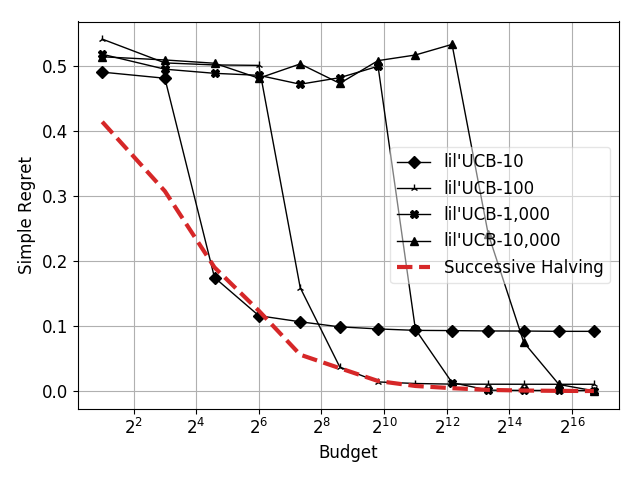
\includegraphics[width=\textwidth]{figures/folder5/alpha1_beta1_unscaled.png}
%	\caption{$Beta(1,1)$}
%	\label{fig:sh-lilucb:alpha1_beta1_unscaled}
%\end{subfigure}
%\quad
%\begin{subfigure}{0.4\textwidth}
%	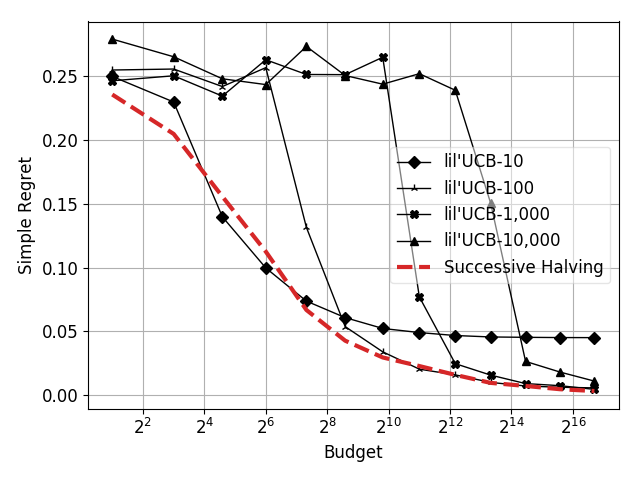
\includegraphics[width=\textwidth]{figures/folder5/alpha1_beta1_scaled.png}
%	\caption{$Beta(1,1)$ Scaled}
%	\label{fig:sh-lilucb:alpha1_beta1_scaled}
%\end{subfigure}
%%
%\begin{subfigure}{0.4\textwidth}
%	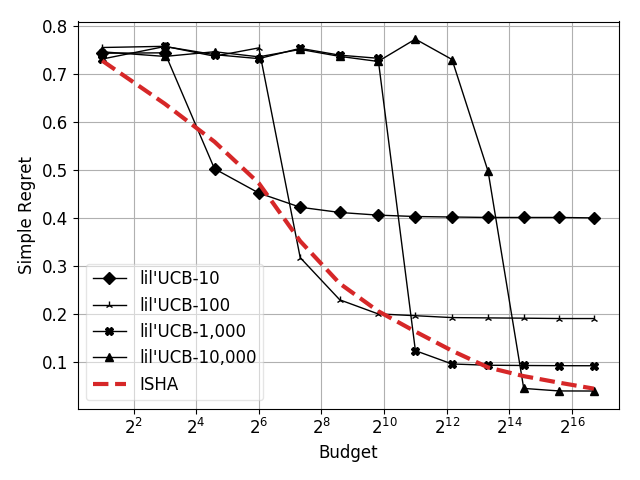
\includegraphics[width=\textwidth]{figures/folder5/alpha1_beta3_unscaled.png}
%	\caption{$Beta(3,1)$}
%	\label{fig:sh-lilucb:alpha1_beta3_unscaled}
%\end{subfigure}
%\quad
%\begin{subfigure}{0.4\textwidth}
%	\includegraphics[width=\textwidth]{figures/folder5/alpha1_beta3_scaled.png}
%	\caption{$Beta(3,1)$ Scaled}
%	\label{fig:sh-lilucb:alpha1_beta3_scaled}
%\end{subfigure}
%%
%%\begin{subfigure}{0.4\textwidth}
%%	\includegraphics[width=\textwidth]{figures/folder5/new_yorker.png}
%%	\caption{New Yorker}
%%	\label{fig:sh-lilucb:new_yorker}
%%\end{subfigure}
%\label{fig:sh-lilucb}
%\end{figure}
%
%
%\begin{figure}
%\centering
%\caption{Comparison to state-of-the-art explore-vs-exploit infinite bandit algorithms}
%\begin{subfigure}{0.4\textwidth}
%	\includegraphics[width=\textwidth]{figures/folder2/alpha1_beta1_unscaled.png}
%	\caption{$Beta(1,1)$}
%	\label{fig:sh-unscaled-alpha1_beta1_unscaled}
%\end{subfigure}
%\quad
%\begin{subfigure}{0.4\textwidth}
%	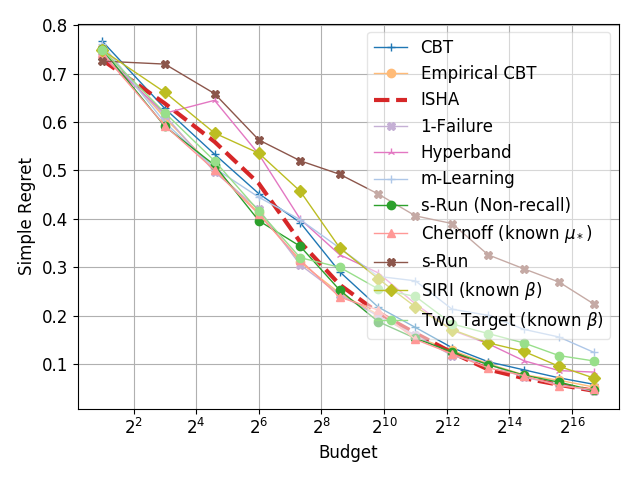
\includegraphics[width=\textwidth]{figures/folder2/alpha1_beta3_unscaled.png}
%	\caption{$Beta(3,1)$}
%	\label{fig:sh-unscaled-alpha1_beta3_unscaled}
%\end{subfigure}
%\label{fig:sh-unscaled}
%\end{figure}
%
%
%\begin{figure}
%\centering
%\caption{Anytime Performance}
%\begin{subfigure}{0.4\textwidth}
%	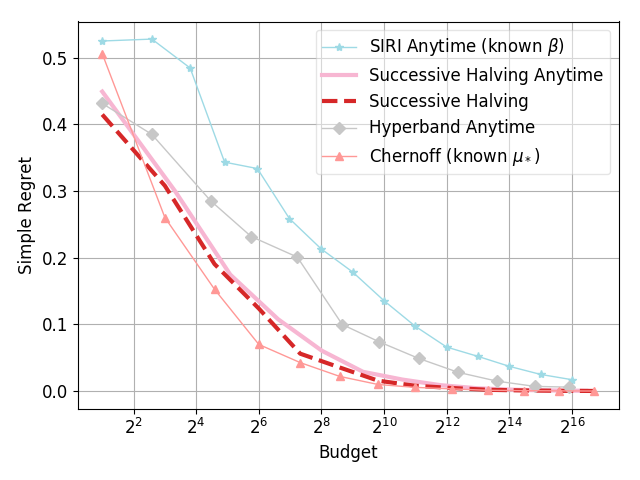
\includegraphics[width=\textwidth]{figures/folder3/alpha1_beta1_unscaled.png}
%	\caption{$Beta(1,1)$}
%	\label{fig:sh-anytime:alpha1_beta1_unscaled}
%\end{subfigure}
%\quad
%\begin{subfigure}{0.4\textwidth}
%	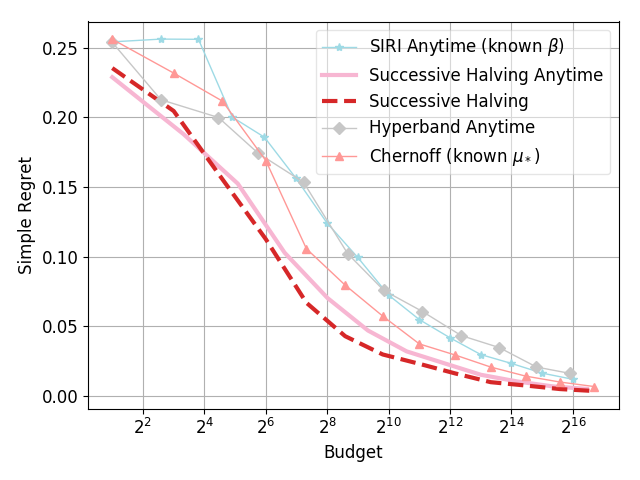
\includegraphics[width=\textwidth]{figures/folder3/alpha1_beta1_scaled.png}
%	\caption{$Beta(1,1)$ Scaled}
%	\label{fig:sh-anytime:alpha1_beta1_scaled}
%\end{subfigure}
%%
%\begin{subfigure}{0.4\textwidth}
%	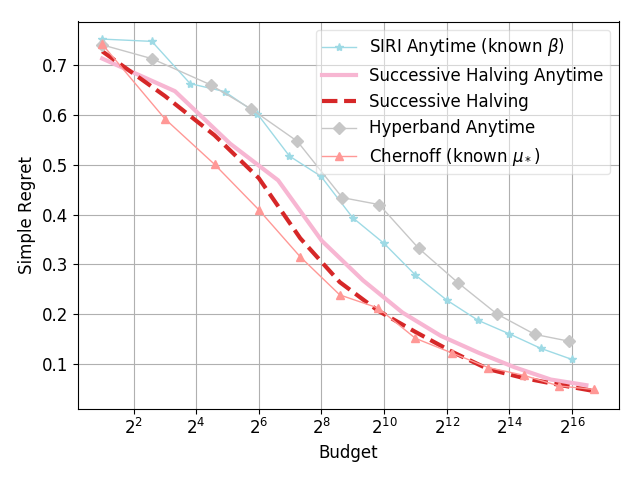
\includegraphics[width=\textwidth]{figures/folder3/alpha1_beta3_unscaled.png}
%	\caption{$Beta(3,1)$}
%	\label{fig:sh-anytime:alpha1_beta3_unscaled}
%\end{subfigure}
%\quad
%\begin{subfigure}{0.4\textwidth}
%	\includegraphics[width=\textwidth]{figures/folder3/alpha1_beta3_scaled.png}
%	\caption{$Beta(3,1)$ Scaled}
%	\label{fig:sh-anytime:alpha1_beta3_scaled}
%\end{subfigure}
%%
%\label{fig:sh-anytime}
%\end{figure}

\clearpage
%\clearpage
%\appendix
%!TEX root = main.tex

\subsection{Additional Proofs}\label{sec:appendix_upper_lemmas}
%\subsubsection{Proof of Lemma~\ref{lem:concentration_in_k}}\label{sec:concentration_in_k_proof}
%\begin{lemma}
%Assume Assumption~\ref{asm:subgauss} holds.
%We have
%\begin{align*}
%\P\left( \bigcup_{\ell=0}^{\log_2(n)-1} \bigcup_{i \in S_{\ell}} \left\{ |\widehat{\mu}_{i,\ell} - \mu_i| \geq \Delta_\ell/2 \right\} \right) \leq \delta/2
%\end{align*}
%\end{lemma}
%\begin{proof}
%By Assumption~\ref{asm:subgauss} and a Chernoff bound, recalling that for the $i$th arm $\widehat{\mu}_{i,\ell}$ is empirical mean of $2^\ell$ i.i.d. draws from $\phi(\mu_i)$, we have 
%\begin{align*}
%\P\left( |\widehat{\mu}_{i,\ell} - \mu_i| \geq \Delta_\ell/2 \right) &\leq 2 \exp( -2^{\ell} (\Delta_\ell/2)^2/2 R ) = 2 \frac{\delta}{n \log_2(n) 2^{-\ell+2}} = \frac{\delta /2}{ |S_\ell| \log_2(n)}
%\end{align*}
%By a union bound and conditioning on the elements in $S_\ell$
%\begin{align*}
%\P\left( \bigcup_{\ell=0}^{\log_2(n)-1} \bigcup_{i \in S_{\ell}} \left\{ |\widehat{\mu}_{i,\ell} - \mu_i| \geq \Delta_\ell/2 \right\} \right)  &\leq \sum_{\ell=0}^{\log_2(n)-1} \E\left[ \P\left( \bigcup_{i \in S_{\ell}} \left\{ |\widehat{\mu}_{i,\ell} - \mu_i| \geq \Delta_\ell/2 \right\} \Big| S_\ell \right) \right] \\ 
%&\leq \sum_{\ell=0}^{\log_2(n)-1} \E\left[  \sum_{i \in S_{\ell}} \P\left( |\widehat{\mu}_{i,\ell} - \mu_i| \geq \Delta_\ell/2 \right) \right] \\
%&\leq \sum_{\ell=0}^{\log_2(n)-1} \E\left[  \sum_{i \in S_{\ell}} \frac{\delta /2}{ |S_\ell| \log_2(n)} \right]  \leq \delta/2
%\end{align*}
%
%\end{proof}
%
%\subsubsection{Proof of Lemma~\ref{lem:good_arms_in_set_k}}\label{sec:good_arms_in_set_k_proof}
%\begin{lemma}
%For any $\ell=0,1,\dots,\log_2(n)-1$ if  $n \geq \xi_{n,\ell} := \frac{\log(2 \log_2(n)/\delta)}{2^{-\ell} \nu_\ell(\mu_* + \Delta_\ell)}$ then 
%% If $n \geq \max_{\ell =0,1,\dots, \log_2(n)-1} \frac{\log(2 \log_2(n)/\delta)}{2^{-\ell} \nu_\ell(\mu_* + \Delta_\ell)}$ then
%\begin{align*}
%\P\left(\min_{i \in S_\ell} \mu_i > \mu_* + \Delta_\ell \right) \leq \tfrac{\delta}{2 \log_2(n)}.
%\end{align*}
%Moreover, $\P\left( \bigcup_{\ell=0}^{\log_2(n)-1} \left\{ \min_{i \in S_\ell} \mu_i > \mu_* + \Delta_\ell \right\} \right)\leq\delta/2$ whenever $n \geq \max_{\ell=0,1,\dots,\log_2(n)-1} \xi_{n,\ell}$.
%\end{lemma}
%\begin{proof}
%By a union bound we have
%\begin{align*}
%\P\left( \bigcup_{\ell=0}^{\log_2(n)-1} \left\{ \min_{i \in S_\ell} \mu_i > \mu_* + \Delta_\ell \right\} \right) 
%&\leq  \sum_{\ell=0}^{\log_2(n)-1} \P(\min_{i \in S_\ell} \mu_i > \mu_* + \Delta_\ell)
%\end{align*}
%so it suffices to show
%\begin{align*}
%\P(\min_{i \in S_\ell} \mu_i > \mu_* + \Delta_\ell) &=
%\E\left[ \P\left( \min_{i \in S_\ell} \mu_i > \mu_* + \Delta_\ell \Big| S_\ell \right) \right] \\
%&=  \P\left( \min_{i =1,\dots, |S_\ell|} \mu_i > \mu_* + \Delta_\ell \Big| \{\mu_i \}_{i=1}^{|S_\ell|} \overset{iid}{\sim} \nu_\ell \right)  \\
%&=  \P\left( \mu_i > \mu_* + \Delta_\ell \Big| \mu_i \overset{iid}{\sim} \nu_\ell \right)^{|S_\ell|} \\
%&=  \left( 1- \nu_\ell( \mu_* + \Delta_\ell) \right)^{|S_\ell|}  \\
%&\leq  \exp\left( - n 2^{-\ell}\nu_\ell( \mu_* + \Delta_\ell) \right) \\
%&\leq  \frac{\delta}{2\log_2(n)}
%\end{align*}
%where the second-to-last line uses the identity $n 2^{-\ell} = |S_\ell|$ and that $1-x \leq e^{-x}$ for all $x\geq0$, and the last line plugs in the assumed condition on $n$.
%\end{proof}
%
%\subsubsection{Proof of Lemma~\ref{lem:core_lemma}} \label{sec:core_lemma_proof}
%\begin{lemma}
%Assume Assumption~\ref{asm:stochastic_ordering} holds.
%For any $k$ and $x\in \R$ we have
%\begin{align*}
%\nu_{k+1}(x) &= 2 \P( \mu_i \in S_{k+1} \, | \, \mu_i \leq x, \mu_i \in S_{k} ) \, \nu_k(x)\\
%&\geq \nu_k(x).
%\end{align*}
%Moreover, for any $k$ and $x < y$ we have $\frac{\nu_{k+1}(x)}{\nu_k(x)} \geq \frac{\nu_{k+1}(y)}{\nu_k(y)}$.
%% \begin{align*}
%% \frac{\nu_{k+1}(x)}{\nu_k(x)} \geq \frac{\nu_{k+1}(y)}{\nu_k(y)}.
%% \end{align*}
%\end{lemma} 
%\begin{proof}
%By Bayes' rule
%\begin{align*}
%\nu_{k+1}(x) &= \P( \mu_i \leq x \, | \, \mu_i \in S_{k+1} )\\
%&= \P( \mu_i \leq x \, | \, \mu_i \in S_{k+1}, \mu_i \in S_{k} )\\
%&= \frac{ \P( \mu_i \in S_{k+1} \, | \, \mu_i \leq x, \mu_i \in S_{k} ) \P( \mu_i \leq x \, | \, \mu_i \in S_{k}) }{ \P(\mu_i \in S_{k+1} \, | \, \mu_i \in S_{k}) }  \\
%&= \nu_k(x) \frac{\P( \mu_i \in S_{k+1} \, | \, \mu_i \leq x, \mu_i \in S_{k} )}{\P(\mu_i \in S_{k+1} \, | \, \mu_i \in S_{k})}.
%\end{align*}
%By definition, $\P(\mu_i \in S_{k+1} \, | \, \mu_i \in S_{k}) = \frac{1}{2}$. 
%On the other hand, ignoring ties (which are broken randomly) we have $\mu_i \in S_{k+1} \iff \widehat{\mu}_{i,k} \leq \tau$.
%Thus, by assumption 1,
%\begin{align*}
%\P( \mu_i \in S_{k+1} \, | \, \mu_i > x, \mu_i \in S_{k} ) \leq \P( \mu_i \in S_{k+1} \, | \, \mu_i \leq x, \mu_i \in S_{k} ).
%\end{align*}
%Applying the law of total probability to $\P(\mu_i \in S_{k+1} \, | \, \mu_i \in S_{k})$ we have
%\begin{align*}
%\hspace{1in}&\hspace{-1in}\frac{\P( \mu_i \in S_{k+1} \, | \, \mu_i \leq x, \mu_i \in S_{k} )}{\P(\mu_i \in S_{k+1} \, | \, \mu_i \in S_{k})}\\
%&= \frac{\P( \mu_i \in S_{k+1} \, | \, \mu_i \leq x, \mu_i \in S_{k} )}{ \nu_k(x) \P( \mu_i \in S_{k+1} \, | \, \mu_i \leq x, \mu_i \in S_{k} ) + (1-\nu_k(x)) \P( \mu_i \in S_{k+1} \, | \, \mu_i > x, \mu_i \in S_{k} )}\\
%&\geq \frac{\P( \mu_i \in S_{k+1} \, | \, \mu_i \leq x, \mu_i \in S_{k} )}{ \nu_k(x) \P( \mu_i \in S_{k+1} \, | \, \mu_i \leq x, \mu_i \in S_{k} ) + (1-\nu_k(x)) \P( \mu_i \in S_{k+1} \, | \, \mu_i \leq x, \mu_i \in S_{k} )} \\
%&= 1.
%\end{align*}
%To obtain the final result, note that
%\begin{align*}
%\frac{\nu_{k+1}(x)}{\nu_k(x)} &= \frac{\P( \mu_i \in S_{k+1} \, | \, \mu_i \leq x, \mu_i \in S_{k} )}{\P(\mu_i \in S_{k+1} \, | \, \mu_i \in S_{k})} \\
%&\geq \frac{\P( \mu_i \in S_{k+1} \, | \, \mu_i \leq y, \mu_i \in S_{k} )}{\P(\mu_i \in S_{k+1} \, | \, \mu_i \in S_{k})} = \frac{\nu_{k+1}(y)}{\nu_k(y)}
%\end{align*}
%\end{proof}

\subsubsection{Proof of Lemma~\ref{lem:exp_N1}}

\begin{proof}
By a manipulation of Wald's identity \cite{WaldsLemma}, if $N$ is a stopping time with finite expectation at which time the procedure declares the arm as $\epsilon$-good or not when run on an arm with mean $\mu$, we have for any $\mu' \neq \mu$
\begin{align}
\E_\mu[N] \geq \frac{\sup_{\mathcal{E}} d( \P_\mu(\mathcal{E}), \P_{\mu'}(\mathcal{E}) )}{KL(\mu,\mu')} \label{eqn:wald}
\end{align}
where $d(x,y) = x \log(\frac{x}{y}) + (1-x) \log(\frac{1-x}{1-y})$.
Now
\begin{align*}
\int_{\mu=\mu_*} \E_\mu[N] d\nu(\mu) &= \int_{\mu=\mu_*}^{\mu_*+\epsilon} \E_\mu[N] d\nu(\mu) + \int_{\mu=\mu_*+\epsilon}^\infty \E_\mu[N] d\nu(\mu) .
\end{align*}


Consider the decomposition $\nu = \nu^a + \nu^s$ where $\nu^a$ and $\nu^s$ are the absolutely continuous and singular components, respectively, of $\nu$ with respect to the Lebesgue measure.
Let $\A^\circ = \{ \{a\} : a \in [\mu_* + \epsilon,\infty) \cap \mathrm{support}(\nu^s),  \frac{d\nu^s(a)}{dx} \geq \kappa \}$ where $\frac{d\nu^s(a)}{dx}$ is the Radon-Nikodym derivative with respect to the Lebesgue measure.
Note that $\A^\circ$ does not contain \emph{all} of the singular components, just those with mass at least $\kappa$.
Let $\A^\perp$ be a collection of disjoint sets that have empty intersection with $\A^\circ$ 
constructed by first covering $[\mu_* + \epsilon,\infty) \cap \mathrm{support}(\nu)-\A^\circ$ with intervals such that $A$ is an interval, $\kappa \leq \nu(A-\A^\circ) \leq 2 \kappa$, and then set $A \leftarrow A \setminus \A^\circ$ such that $A$ is an interval in all but a set of measure $0$.
Finally, define $\A = \A^\circ \cup \A^\perp$.
Note that $\min_{A \in \A} \nu(A) \geq \kappa$.
Also note that for any $A \in \A$ we have $\sup_{x,y \in A} |x-y| > 0$ if and only if $A \in \A^\perp$ so that we also have $\nu(A) \leq 2 \kappa$.  


% Fix $\kappa \in (0,1)$. 
% Let $t_0 = \mu_* + \epsilon$ and let $\A =\{A_1,A_2,\dots\}$ where $A_k = (t_{k-1}, t_k]$ and $t_k = \min\{ t : \nu(t) \geq \nu(t_{k-1}) + \kappa\}$ so that $\nu(A_k) \geq \kappa$ and $A_{k+1} = \arg\sup_{A \subset \R \setminus \{A_{\ell}\}_{\ell < k}: \nu(A)\geq \kappa} \frac{\nu(A)}{\sup_{x \in A} KL(\mu_*, x)}$
% Inflate the last set so that so that it contains the support. 

Let $E$ denote the event that the current arm is the declared as $\epsilon$-good.
Given such a partition, note that
\begin{align*}
\max_{A \in \A} \frac{1}{\nu(A)} \int_{\mu \in A} \P_\mu(E) d\nu(\mu) &\leq \sum_{A \in \A} \frac{1}{\nu(A)} \int_{\mu \in A} \P_\mu(E) d\nu(\mu) \\
&\leq \frac{1}{\kappa} \sum_{A \in \A} \int_{\mu \in A} \P_\mu(E) d\nu(\mu) \\
&= \frac{1}{\kappa} \int_{\mu = \mu_* + \epsilon} \P_\mu(E) d\nu(\mu) \\
&=  \frac{\alpha(1-\pi)}{\kappa}  \\
&< 1-\beta
\end{align*}
where the last line holds by assumption.
By the definition of $\widetilde{\mu}$ in the statement, if $\widetilde{A} = (\mu_*+\epsilon, \widetilde{\mu}]$ then $\nu(\widetilde{A}) \geq \kappa$ so
\begin{align*}
\int_{\mu=\mu_*}^{\mu_*+\epsilon} \E_\mu[N] d\nu(\mu) &= \pi \frac{1}{\nu(\widetilde{A})}  \int_{\mu' \in \widetilde{A}} \frac{1}{\pi} \int_{\mu=\mu_*}^{\mu_*+\epsilon} \E_\mu[N] d\nu(\mu) d\nu(\mu')\\
&\overset{(i)}{\geq} \pi  \frac{1}{\nu(\widetilde{A})} \int_{\mu' \in \widetilde{A}} \frac{1}{\pi} \int_{\mu=\mu_*}^{\mu_*+\epsilon} \frac{d( \P_\mu(E), \P_{\mu'}(E) )}{KL(\mu,\mu')}  d\nu(\mu) d\nu(\mu') \\
&\overset{(ii)}{\geq} \pi  \frac{1}{KL(\mu_*,\widetilde{\mu})} \frac{1}{\nu(\widetilde{A})} \int_{\mu' \in \widetilde{A}} \frac{1}{\pi} \int_{\mu=\mu_*}^{\mu_*+\epsilon} d( \P_\mu(E), \P_{\mu'}(E) )  d\nu(\mu) d\nu(\mu') \\
&\overset{(iii)}{\geq}  \pi  \frac{1}{KL(\mu_*,\widetilde{\mu})} d\left( \frac{1}{\pi} \int_{\mu=\mu_*}^{\mu_*+\epsilon} \P_\mu(E)d\nu(\mu) , \frac{1}{\nu(\widetilde{A})} \int_{\mu' \in \widetilde{A}}  \P_{\mu'}(E) d\nu(\mu') \right)    \\
&\overset{(iv)}{\geq} \pi  d(1-\beta,  \tfrac{\alpha(1-\pi)}{\nu(\widetilde{A})}) \frac{1}{KL(\mu_*,\widetilde{\mu})} 
\end{align*}
where $(i)$ follows from Equation~\ref{eqn:wald}, 
$(ii)$ uses the fact that $KL(a,b) \leq KL(c,d)$ whenever $[a,b] \subseteq [c,d]$, 
$(iii)$ uses the fact that binary KL divergence is convex \cite{Cover:2006:EIT:1146355}, 
and $(iv)$ holds because $\max_{A \in \A} \frac{1}{\nu(A)}\int_{\mu \in A} \P_\mu(E) d\nu(\mu) \leq \frac{\alpha(1-\pi)}{\kappa} < 1-\beta$ by assumption.


The second term follows analogously
\begin{align*}
\int_{\mu=\mu_*+\epsilon}^\infty \E_\mu[N] d\nu(\mu) &= \sum_{A \in \A} \nu(A) \frac{1}{\nu(A)} \int_{\mu \in A} \E_\mu[N] d\nu(\mu) \\
&= \sum_{A \in \A} \nu(A) \frac{1}{\pi}\int_{\mu' =\mu_*}^{\mu_* + \epsilon} \frac{1}{\nu(A)} \int_{\mu \in A} \E_\mu[N] d\nu(\mu) d\nu(\mu')\\
&\overset{(i)}{\geq} \sum_{A \in \A} \nu(A)\frac{1}{\pi}\int_{\mu' =\mu_*}^{\mu_* + \epsilon} \frac{1}{\nu(A)} \int_{\mu \in A} \frac{d( \P_\mu(E), \P_{\mu'}(E) )}{KL(\mu,\mu')}  d\nu(\mu) d\nu(\mu') \\
&\overset{(ii)}{\geq} \sum_{A \in \A}  \frac{\nu(A)}{\sup_{\mu \in A} KL(\mu,\mu_*)} \frac{1}{\pi}\int_{\mu' =\mu_*}^{\mu_* + \epsilon}\frac{1}{\nu(A)} \int_{\mu \in A} d( \P_\mu(E), \P_{\mu'}(E) )  d\nu(\mu) d\nu(\mu') \\
&\overset{(iii)}{\geq} \sum_{A \in \A} \frac{\nu(A)}{\sup_{\mu \in A} KL(\mu,\mu_*)} d\left( \frac{1}{\nu(A)}\int_{\mu \in A}  \P_\mu(E) d\nu(\mu) , \frac{1}{\pi}\int_{\mu' =\mu_*}^{\mu_* + \epsilon} \P_{\mu'}(E) d\nu(\mu')\right)  \\
&\overset{(iv)}{\geq} d\left( \tfrac{\alpha(1-\pi)}{\kappa} , 1-\beta \right) \sum_{A \in \A}  \frac{\nu(A)}{\sup_{\mu \in A} KL(\mu,\mu_*)}  
\end{align*}
where $(i)-(iv)$ follow for identical reasons as above.

Index the sets of $\A^\perp$ into $A_1,A_2,\dots,A_{|\A^\perp|}$ where $\sup_{x \in A_k} x \leq \inf_{y \in A_{k+1}} y$ for all $k$. 
Recalling that $\sup_{x \in A} x = \inf_{x \in A} x$ for all $A \in \A^\circ$ and $\kappa \leq \nu(A) \leq 2\kappa$ for all $A \in \A^\perp$ we have 
\begin{align*}
\sum_{A \in \A}  \frac{\nu(A)}{\sup_{\mu \in A} KL(\mu,\mu_*)} 
&= \sum_{k = 1}^{|\A^\perp|}  \frac{\nu(A_k)}{\sup_{\mu \in A_k} KL(\mu,\mu_*)} + \sum_{A \in \A^\circ}  \frac{\nu(A)}{\inf_{\mu \in A} KL(\mu,\mu_*)} \\
&\geq \sum_{k = 1}^{|\A^\perp|-1}  \frac{\nu(A_{k+1})/2}{\sup_{\mu \in A_k} KL(\mu,\mu_*)} + \sum_{A \in \A^\circ}  \frac{\nu(A)}{\inf_{\mu \in A} KL(\mu,\mu_*)} \\
&\geq \sum_{k = 1}^{|\A^\perp|-1}  \frac{\nu(A_{k+1})/2}{\inf_{\mu \in A_{k+1}} KL(\mu,\mu_*)} + \sum_{A \in \A^\circ}  \frac{\nu(A)}{\inf_{\mu \in A} KL(\mu,\mu_*)} \\
% &=  \frac{\nu(A_1)}{\sup_{\mu \in A_1} KL(\mu,\mu_*)} + \sum_{A_k \in \A^\perp \setminus A_{1}}  \frac{\nu(A_{k})}{\sup_{\mu \in A_{k}} KL(\mu,\mu_*)} + \sum_{A \in \A^\circ}  \frac{\nu(A)}{\inf_{\mu \in A} KL(\mu,\mu_*)} \\
% &\geq  \frac{\nu(A_2)/2}{\sup_{\mu \in A_1} KL(\mu,\mu_*)} + \sum_{A_k \in \A^\perp \setminus A_{1}}  \frac{\nu(A_{k})}{\sup_{\mu \in A_{k}} KL(\mu,\mu_*)} + \sum_{A \in \A^\circ}  \frac{\nu(A)}{\inf_{\mu \in A} KL(\mu,\mu_*)} \\
% &\geq  \frac{\nu(A_2)/2}{\inf_{\mu \in A_2} KL(\mu,\mu_*)} + \sum_{A_k \in \A^\perp \setminus A_{1}}  \frac{\nu(A_{k})}{\sup_{\mu \in A_{k}} KL(\mu,\mu_*)} + \sum_{A \in \A^\circ}  \frac{\nu(A)}{\inf_{\mu \in A} KL(\mu,\mu_*)} \\
&=   \sum_{k = 2}^{|\A^\perp|}  \frac{\nu(A_k)/2}{\inf_{\mu \in A_k} KL(\mu,\mu_*)} + \sum_{A \in \A^\circ}  \frac{\nu(A)}{\inf_{\mu \in A} KL(\mu,\mu_*)}\\
&=  -\frac{\nu(A_1)/2}{\inf_{\mu \in A_1} KL(\mu,\mu_*)} + \sum_{A \in \A}  \frac{\nu(A)/2}{\inf_{\mu \in A} KL(\mu,\mu_*)}\\
&\geq   -\frac{\kappa}{KL(\mu_*+\epsilon,\mu_*)}  + \frac{1}{2} \int_{\mu_*+\epsilon} \frac{1}{KL(\mu,\mu_*)} d\nu(\mu) 
 \end{align*}
 % We immediately have $\frac{\nu(A_1)/2}{\inf_{\mu \in A_1} KL(\mu,\mu_*)} \leq \frac{\kappa}{KL(\mu_*+\epsilon,\mu_*)}$.
 % However, we can get a tighter representation by considering the definition of $A_1$.
% While $A_1$ may contain a singular component we also know $\nu^s(A_1) + \nu^a(A_1) \leq 2\kappa$ so we clearly have $\sup\{\mu:\mu \in A_1\} \leq \dot{\mu}$ where $\dot{\mu} = \sup\{ \mu : \nu^a(\mu) - \nu^a(\mu_*+\epsilon) \leq 2\kappa \}$
%  so that
%  \begin{align*}
%  -\frac{\nu(A_1)/2}{\inf_{\mu \in A_1} KL(\mu,\mu_*)}  + \frac{1}{2} \int_{\mu_*+\epsilon} \frac{1}{KL(\mu,\mu_*)} d\nu(\mu) \geq \frac{1}{2} \int_{\dot{\mu}} \frac{1}{KL(\mu,\mu_*)} d\nu(\mu)
%  \end{align*}
%  Trivially we have
%  \begin{align*}
%  \int_{\dot{\mu}} \frac{1}{KL(\mu,\mu_*)} d\nu(\mu) \geq \frac{-2\kappa}{KL(\mu_*+\epsilon,\mu_*)} + \int_{\mu_*+\epsilon} \frac{1}{KL(\mu,\mu_*)} d\nu(\mu)
%  \end{align*}
so that
 \begin{align*}
 \int_{\mu=\mu_*+\epsilon}^\infty \E_\mu[N] d\nu(\mu) \geq d\left( \tfrac{\alpha(1-\pi)}{\kappa}, 1-\beta \right) \left(  - \frac{\kappa}{KL(\mu_* + \epsilon, \mu_*)}  + \frac{1}{2} \int_{\mu_*+\epsilon} \frac{1}{KL(\mu,\mu_*)} d\nu(\mu) \right).
 \end{align*}
 \end{proof}

\subsubsection{Proof of Theorem~\ref{thm:fb-lb}}

\begin{proof}
We plug in the result of Lemma~\ref{lem:exp_N1} with $\kappa=2\pi$ into Equation~\ref{eqn:N1_to_many} to obtain
\begin{align*}
\E[ \sum_{i \geq 1} N_i ] \geq& \pi \frac{ d\left(1-\beta,  \tfrac{\alpha(1-\pi)}{\widetilde{\kappa}}\right) }{\alpha (1-\pi) + (1-\beta) \pi} \frac{1}{KL(\mu_*,\widetilde{\mu})}  \\
&+\frac{
d\left(\tfrac{\alpha(1-\pi)}{\kappa} , 1-\beta \right)}{\alpha (1-\pi) + (1-\beta) \pi} \left(  - \frac{\kappa}{KL(\mu_* + \epsilon, \mu_*)}  + \frac{1}{2} \int_{\mu_*+\epsilon} \frac{1}{KL(\mu,\mu_*)} d\nu(\mu) \right).
\end{align*}

For the first term we apply the assumption $\frac{(1-\pi)\alpha}{\pi(1-\beta)} \leq \frac{\delta}{1-\delta}$  to obtain
\begin{align*}
\frac{\pi \, d(1-\beta,  \tfrac{\alpha(1-\pi)}{\widetilde{\kappa}})}{\alpha (1-\pi) + (1-\beta) \pi} &\geq \frac{d(1-\beta, \tfrac{\delta \pi}{(1-\delta)\widetilde{\kappa}} (1-\beta))}{(1-\beta) /(1-\delta)} \\
&= \frac{(1-\beta) \log(\tfrac{(1-\delta)\widetilde{\kappa}}{\delta \pi}) + \beta \log(\beta)  - \beta \log(1-\tfrac{\delta \pi (1-\beta)}{(1-\delta)\kappa})}{(1-\beta) /(1-\delta)} \\
&\geq (1-\delta) \log(\tfrac{(1-\delta)\widetilde{\kappa}}{\delta \pi}) + (1-\delta) \tfrac{\beta}{1-\beta} \log(\beta) \\
&\geq (1-\delta) \log(\tfrac{(1-\delta)\widetilde{\kappa}}{\delta e}) 
\end{align*}
using the fact that $-\tfrac{\beta}{1-\beta} \log(\beta) \in (0,1)$ for $\beta \in (0,1)$.

For the second term we apply the assumption again to get
\begin{align*}
\frac{d\left(\tfrac{\alpha(1-\pi)}{\kappa} , 1-\beta \right)}{\alpha (1-\pi) + (1-\beta) \pi} &\geq \frac{d\left(\tfrac{\pi \delta}{\kappa (1-\delta)} (1-\beta) , 1-\beta \right)}{(1-\beta) \pi/(1-\delta)} \\
&= \frac{ \tfrac{\pi \delta}{\kappa (1-\delta)} (1-\beta) \log(\tfrac{\pi \delta}{\kappa (1-\delta)}) + \left(1- \tfrac{\pi \delta}{\kappa (1-\delta)} (1-\beta)\right) \log( \frac{1- \tfrac{\pi \delta}{\kappa (1-\delta)} (1-\beta)}{\beta})}{(1-\beta) \pi/(1-\delta)} \\
&= \tfrac{1-\delta}{\pi} \tfrac{\pi \delta}{\kappa (1-\delta)}  \log(\tfrac{\pi \delta}{\kappa (1-\delta)}) + \tfrac{1-\delta}{\pi}\left(1- \tfrac{\pi \delta}{\kappa (1-\delta)} (1-\beta)\right)\left( \tfrac{\log(1/\beta)}{1-\beta} + \tfrac{\log\left( 1- \tfrac{\pi \delta}{\kappa (1-\delta)} (1-\beta) \right)}{1-\beta} \right)\\
&\geq \tfrac{1-\delta}{\pi} \tfrac{\delta/2}{1-\delta}  \log(\tfrac{\delta/2}{1-\delta}) + \tfrac{1-\delta}{\pi}\left(1- \tfrac{\delta /2}{ 1-\delta} (1-\beta)\right)\left( 1- \tfrac{\delta}{1-\delta}   \right) \\
&\geq \tfrac{1-\delta}{\pi}( 1 + \tfrac{\delta/2}{1-\delta}  \log(\tfrac{\delta/2}{1-\delta}) - \tfrac{3\delta/2}{1-\delta} ) \\
&\geq \tfrac{1 - \tfrac{\delta}{2}  \log(\tfrac{1-\delta}{\delta/42})}{\pi} 
\end{align*}
where the last lines use $\kappa = 2\pi$, $\tfrac{\log(1/\beta)}{1-\beta} \geq 1$ for all $\beta \in (0,1)$, $\log(1-x) \geq -2x$ for $x \in (0,1/2)$, and $\delta \in (0, 12]$.
Thus, putting the pieces together we obtain
\begin{align*}
\E[ \sum_{i \geq 1} N_i ] &\geq \frac{(1-\delta) \log(\tfrac{(1-\delta)\widetilde{\kappa}}{\delta \pi e})}{KL(\mu_* , \widetilde{\mu})} + \tfrac{1 - \tfrac{\delta}{2}  \log(\tfrac{1-\delta}{\delta/42})}{\pi} \left(  - \frac{ \kappa}{KL(\mu_* + \epsilon, \mu_*)}  + \frac{1}{2} \int_{\mu_*+\epsilon} \frac{1}{KL(\mu,\mu_*)} d\nu(\mu) \right) \\
&= \frac{ (1-\delta) \log(\tfrac{(1-\delta)\widetilde{\kappa}}{\delta \pi e})}{KL(\mu_* , \widetilde{\mu})}  + (1 - \tfrac{\delta}{2}  \log(\tfrac{1-\delta}{\delta/42})) \left(  - \frac{2}{KL(\mu_* + \epsilon, \mu_*)}  + \frac{1}{2\pi} \int_{\mu_*+\epsilon} \frac{1}{KL(\mu,\mu_*)} d\nu(\mu) \right).
\end{align*}
Finally, $1 \geq (1 - \tfrac{\delta}{2}  \log(\tfrac{1-\delta}{\delta/42}))\geq 3/4$ for $\delta \leq 1/15$.

\end{proof}

\subsection {Empirical study}\label{appendix:experiments}

Here we present further results in addition to what we provided in Section~\ref{experiments}. We start with describing in some detail the baselines we used and then present further experiments on various reservoirs.

\textbf{Pure exploration algorithms.}
Our first batch of baselines are pure exploration algorithms.

We introduce the algorithm we call Chernoff, meant as a strong baseline
for ISHA. This algorithm has knowledge of $\mu_*$.
We define the algorithm in terms of the confidence lower bound $L_i(t) = \min \{q \in [0,\widehat{\mu}_{i}] : N_i(t) KL(\hat{\mu}_i(t),q) \le \log(1/\delta_k) \}\label{kl-ub}$
where $t$ is the budget used so far,
$N_i(t)$ is the number of times arm $i$ is pulled,
and $\delta_k = \frac{6\delta}{(\pi N_i(t))^2}$ for $\delta=0.1$ so that the overall error tolerance for an arm $i$ is $\delta$.
This algorithm draws an arm from the reservoir and continues drawing
rewards from it until $L_i(t) > \mu_*$. Once its confidence interval no longer contains $\mu_*$, the arm is discarded and a new arm is drawn.
At time $T$ the algorithm stops and returns the arm that was sampled the most. 

SIRI \citep{DBLP:journals/corr/CarpentierV15} is a recent UCB-style pure exploration algorithm in the fixed budget setting.
It is based on a $\beta$-regularity assumption for the tail of the
reservoir, and so makes use of additional information about the reservoir.
We run this with $\delta=0.1$.

lil'UCB \citep{Jamieson2014lilU}, another UCB algorithm, is a fixed confidence pure exploration algorithm for finite bandits. While the original lil'UCB has its own stopping criterion, in our experiments it stops when it runs out of budget. For consistency, we use the $L_i(t)$ defined for Chernoff with the same $\delta$ value and schedule used therein.

We also run Hyperband~\citep{li2017hyperband}, described earlier.
Its parameter $\eta$ decides which fraction of arms to discard in a given round of Successive Halving. We used $\eta=2$ (discarding half the arms) in keeping with Successive Halving.

Successive Rejects \citep{DBLP:conf/colt/AudibertBM10}, a fixed budget algorithm originally intended for finite bandits, is similar to Successive Halving. We run it with $n^*_T$ arms. 

\paragraph{Explore-vs-Exploit algorithms.}
We use regret minimization infinite bandit algorithms
as our next batch of baselines.
Note that these algorithms are not natural competitors and do not have an arm recommendation strategy. At time $T$ we stop and return the arm that was sampled the most.

We  experiment with four infinite bandit algorithms of \cite{berry1997} designed for $Beta(1,1)$ with support on $[0,1]$:
$f$-failure strategy (with $f=1$) which samples an arm until
$f$ failures are observed,
$s$-run strategy (with $s=\sqrt{T}$) which samples each arm
at most $s$ times until a failure is observed and then exploits the most
successful arm until the budget is exhausted,
$s$-run strategy (non-recall; $s=\sqrt{T}$) which samples from
an arm until the first failure but exploits the arm until the budget
is exhausted if $s$ successes are observed, and
$m$-learning strategy (with $m=\log(T)\sqrt{T}$) which plays the $f$-failure strategy (with $f=1$) for the first $m$
times (the arm at time $m$ is exploited until a failure is observed). From there the empirically-best arm is exploited. 

CBT and Empirical CBT  
\cite{Chan2018Infinite} are also used as baselines.
CBT takes as input a target mean parameter $\mu_{target}=\sqrt{2/T}$ for reservoir $Beta(1,1)$, and $\mu_{target}=\sqrt[4]{4/T}$ for $Beta(3,1)$  and thus assumes
knowledge of the reservoir.
Empirical CBT does not assume anything about the reservoir but
instead estimates $\mu_{target}$. 

Two Target (fixed horizon) \cite{bonald2013two} uses
two success target thresholds
$l_1$ and $l_2$ as function of the reservoir parameters $\beta$ and $\alpha$, and budget $T$.
Any arm which fails to have $l_1$ 
successes before its first failure is discarded,
and any arm which has $l_2$ successes before its first $m$ failures
is subsequently exploited until the budget is exhausted.
We use $m=3$ in our experiments.  


\paragraph{Anytime algorithms.}
We also propose the following Anytime version
of ISHA and compare it to other anytime algorithms.
When an effectively unlimited budget is available, ISHA
Anytime can be run as follows.
Choose increasing dyadic numbers of arms, $n=2^i, i=1,2,\dots$.
For each value of $n$, sample $n$ new arms and
run ISHA and save the result
as the best arm found so far.
We compare this algorithm to Hyperband Anytime and SIRI Anytime (using the budget doubling trick as proposed by the SIRI authors).

\subsubsection{Experiments and Insights}\label{appendix:fb-experiments}
\paragraph{Successive Halving performance as a function of the number of arms for a fixed budget.}
The class of experiments in Figure~\ref{appendix:fig:sh-num-arms} reports the average simple regret for ISHA (Successive Halving using the maximum number of arms s.t. $T \ge n^*_T\log_2 n^*_T$) in comparison to various
smaller choices of $n$. Across a variety of reservoirs, $n^*_T$ arms is always a good choice for Successive Halving in the infinite setting.

\paragraph{Simple regret vs. Budget.} 
In the class of experiments in Figure~\ref{appendix:fig:sh-infinite} we compare the simple regret of
ISHA to that of various pure exploration baselines.
 
Figure~\ref{appendix:fig:sh-lilucb} highlights the difficulty of
choosing the optimal number of arms for UCB-style algorithms,
such as the lil'UCB.

Figure~\ref{appendix:fig:sh-unscaled} compares mainly against various exploration-vs-exploitation baselines, some of which were specifically designed specifically for $Beta$ reservoirs.

Finally, in Figure~\ref{appendix:fig:sh-anytime}, we compare ISHA  and ISHA Anytime to several other anytime algorithms.

\clearpage

\begin{figure}
\centering
\caption{Impact of the number of arms for a fixed budget and reservoir.}
\begin{subfigure}{0.4\textwidth}
	\includegraphics[width=\textwidth]{fixedbudget/figures/folder1/alpha1_beta1_unscaled.png}
	\caption{$Beta(1,1)$}
	\label{appendix:fig:sh-num-arms:alpha1_beta1_unscaled}
\end{subfigure}
\quad
\begin{subfigure}{0.4\textwidth}
	\includegraphics[width=\textwidth]{fixedbudget/figures/folder1/alpha1_beta1_scaled.png}
	\caption{$Beta(1,1)$ Scaled}
	\label{appendix:fig:sh-num-arms:alpha1_beta1_scaled}
\end{subfigure}
%
\begin{subfigure}{0.4\textwidth}
	\includegraphics[width=\textwidth]{fixedbudget/figures/folder1/alpha1_beta3_unscaled.png}
	\caption{$Beta(3,1)$}
	\label{appendix:fig:sh-num-arms:alpha1_beta3_unscaled}
\end{subfigure}
\quad
\begin{subfigure}{0.4\textwidth}
	\includegraphics[width=\textwidth]{fixedbudget/figures/folder1/alpha1_beta3_scaled.png}
	\caption{$Beta(3,1)$ Scaled}
	\label{appendix:fig:sh-num-arms:alpha1_beta3_scaled}
\end{subfigure}
%
\begin{subfigure}{0.4\textwidth}
	\includegraphics[width=\textwidth]{fixedbudget/figures/folder1/{TwoSpike_0.1_0.515_0.031}.png}
	\caption{TwoSpike $\pi=10^{-1}, \epsilon=\sqrt{10^{-3}}$}
	\label{appendix:fig:sh-num-arms:TwoSpike_1}
\end{subfigure}
\quad
\begin{subfigure}{0.4\textwidth}
	\includegraphics[width=\textwidth]{fixedbudget/figures/folder1/{TwoSpike_0.01_0.55_0.1}.png}
	\caption{Two Spike $\pi=10^{-2}, \epsilon=\sqrt{10^{-2}}$}
	\label{appendix:fig:sh-num-arms:TwoSpike_2}
\end{subfigure}
%
\begin{subfigure}{0.4\textwidth}
	\includegraphics[width=\textwidth]{fixedbudget/figures/folder1/{TwoSpike_0.001_0.658_0.316}.png}
	\caption{Two Spike $\pi=10^{-3}, \epsilon=\sqrt{10^{-1}}$}
	\label{appendix:fig:sh-num-arms:TwoSpike_3}
\end{subfigure}
\quad
\begin{subfigure}{0.4\textwidth}
	\includegraphics[width=\textwidth]{fixedbudget/figures/folder1/new_yorker.png}
	\caption{New Yorker}
	\label{appendix:fig:sh-num-arms:new_yorker}
\end{subfigure}
\label{appendix:fig:sh-num-arms}
\end{figure}

\begin{figure}
\centering
\caption{Comparison to state-of-the-art pure exploration infinite bandit algorithms}
\begin{subfigure}{0.4\textwidth}
	\includegraphics[width=\textwidth]{fixedbudget/figures/folder4/alpha1_beta1_unscaled.png}
	\caption{$Beta(1,1)$}
	\label{appendix:fig:sh-infinite:alpha1_beta1_unscaled}
\end{subfigure}
\quad
\begin{subfigure}{0.4\textwidth}
	\includegraphics[width=\textwidth]{fixedbudget/figures/folder4/alpha1_beta1_scaled.png}
	\caption{$Beta(1,1)$ Scaled}
	\label{appendix:fig:sh-infinite:alpha1_beta1_scaled}
\end{subfigure}
%
\begin{subfigure}{0.4\textwidth}
	\includegraphics[width=\textwidth]{fixedbudget/figures/folder4/alpha1_beta3_unscaled.png}
	\caption{$Beta(3,1)$}
	\label{appendix:fig:sh-infinite:alpha1_beta3_unscaled}
\end{subfigure}
\quad
\begin{subfigure}{0.4\textwidth}
	\includegraphics[width=\textwidth]{fixedbudget/figures/folder4/alpha1_beta3_scaled.png}
	\caption{$Beta(3,1)$ Scaled}
	\label{appendix:fig:sh-infinite:alpha1_beta3_scaled}
\end{subfigure}
%
\begin{subfigure}{0.4\textwidth}
	\includegraphics[width=\textwidth]{fixedbudget/figures/folder4/{TwoSpike_0.1_0.515_0.031}.png}
	\caption{TwoSpike $\pi=10^{-1}, \epsilon=\sqrt{10^{-3}}$}
	\label{appendix:fig:sh-infinite:TwoSpike_1}
\end{subfigure}
\quad
\begin{subfigure}{0.4\textwidth}
	\includegraphics[width=\textwidth]{fixedbudget/figures/folder4/{TwoSpike_0.01_0.55_0.1}.png}
	\caption{Two Spike $\pi=10^{-2}, \epsilon=\sqrt{10^{-2}}$}
	\label{appendix:fig:sh-infinite:TwoSpike_2}
\end{subfigure}
%
\begin{subfigure}{0.4\textwidth}
	\includegraphics[width=\textwidth]{fixedbudget/figures/folder4/{TwoSpike_0.001_0.658_0.316}.png}
	\caption{Two Spike $\pi=10^{-3}, \epsilon=\sqrt{10^{-1}}$}
	\label{appendix:fig:sh-infinite:TwoSpike_3}
\end{subfigure}
\quad
\begin{subfigure}{0.4\textwidth}
	\includegraphics[width=\textwidth]{fixedbudget/figures/folder4/new_yorker.png}
	\caption{New Yorker}
	\label{appendix:fig:sh-infinite:new_yorker}
\end{subfigure}
\label{appendix:fig:sh-infinite}
\end{figure}


\begin{figure}
\centering
\caption{Comparison to lil'UCB}
\begin{subfigure}{0.4\textwidth}
	\includegraphics[width=\textwidth]{fixedbudget/figures/folder5/alpha1_beta1_unscaled.png}
	\caption{$Beta(1,1)$}
	\label{appendix:fig:sh-lilucb:alpha1_beta1_unscaled}
\end{subfigure}
\quad
\begin{subfigure}{0.4\textwidth}
	\includegraphics[width=\textwidth]{fixedbudget/figures/folder5/alpha1_beta1_scaled.png}
	\caption{$Beta(1,1)$ Scaled}
	\label{appendix:fig:sh-lilucb:alpha1_beta1_scaled}
\end{subfigure}
%
\begin{subfigure}{0.4\textwidth}
	\includegraphics[width=\textwidth]{fixedbudget/figures/folder5/alpha1_beta3_unscaled.png}
	\caption{$Beta(3,1)$}
	\label{appendix:fig:sh-lilucb:alpha1_beta3_unscaled}
\end{subfigure}
\quad
\begin{subfigure}{0.4\textwidth}
	\includegraphics[width=\textwidth]{fixedbudget/figures/folder5/alpha1_beta3_scaled.png}
	\caption{$Beta(3,1)$ Scaled}
	\label{appendix:fig:sh-lilucb:alpha1_beta3_scaled}
\end{subfigure}
%
%\begin{subfigure}{0.4\textwidth}
%	\includegraphics[width=\textwidth]{figures/folder5/new_yorker.png}
%	\caption{New Yorker}
%	\label{fig:sh-lilucb:new_yorker}
%\end{subfigure}
\label{appendix:fig:sh-lilucb}
\end{figure}


\begin{figure}
\centering
\caption{Comparison to state-of-the-art explore-vs-exploit infinite bandit algorithms}
\begin{subfigure}{0.4\textwidth}
	\includegraphics[width=\textwidth]{fixedbudget/figures/folder2/alpha1_beta1_unscaled.png}
	\caption{$Beta(1,1)$}
	\label{appendix:fig:sh-unscaled-alpha1_beta1_unscaled}
\end{subfigure}
\quad
\begin{subfigure}{0.4\textwidth}
	\includegraphics[width=\textwidth]{fixedbudget/figures/folder2/alpha1_beta3_unscaled.png}
	\caption{$Beta(3,1)$}
	\label{appendix:fig:sh-unscaled-alpha1_beta3_unscaled}
\end{subfigure}
\label{appendix:fig:sh-unscaled}
\end{figure}


\begin{figure}
\centering
\caption{Anytime Performance}
\begin{subfigure}{0.4\textwidth}
	\includegraphics[width=\textwidth]{fixedbudget/figures/folder3/alpha1_beta1_unscaled.png}
	\caption{$Beta(1,1)$}
	\label{appendix:fig:sh-anytime:alpha1_beta1_unscaled}
\end{subfigure}
\quad
\begin{subfigure}{0.4\textwidth}
	\includegraphics[width=\textwidth]{fixedbudget/figures/folder3/alpha1_beta1_scaled.png}
	\caption{$Beta(1,1)$ Scaled}
	\label{appendix:fig:sh-anytime:alpha1_beta1_scaled}
\end{subfigure}
%
\begin{subfigure}{0.4\textwidth}
	\includegraphics[width=\textwidth]{fixedbudget/figures/folder3/alpha1_beta3_unscaled.png}
	\caption{$Beta(3,1)$}
	\label{appendix:fig:sh-anytime:alpha1_beta3_unscaled}
\end{subfigure}
\quad
\begin{subfigure}{0.4\textwidth}
	\includegraphics[width=\textwidth]{fixedbudget/figures/folder3/alpha1_beta3_scaled.png}
	\caption{$Beta(3,1)$ Scaled}
	\label{appendix:fig:sh-anytime:alpha1_beta3_scaled}
\end{subfigure}
%
\label{appendix:fig:sh-anytime}
\end{figure}

\begin{figure}
% \vspace{-2.5em}
\includegraphics[width=\textwidth]{fixedbudget/figures/NY_CDF.pdf}
\caption{New Yorker CDF}
\label{fig:newyorkercdf}
\end{figure}

\clearpage

%\end{document}

